%% Copernicus Publications Manuscript Preparation Template for LaTeX Submissions
\documentclass[gmd, manuscript]{copernicus} %final manuscript
\usepackage{url}
\Urlmuskip=0mu plus 1mu % for better line break in very long globus URLs

%\externaldocument{../PhaseIIPaper/Part1/supdocs/supdoc}

\begin{document}
\title{The GGCMI Phase II experiment: global gridded crop model simulations under uniform changes in CO$_2$, temperature, water, and nitrogen levels (protocol version 1.0)}

\Author[1,2]{James}{Franke}
\Author[3]{Christoph}{M\"{u}ller}
\Author[2,4]{Joshua}{Elliott}
\Author[5]{Alex C.}{Ruane}
\Author[6]{Abigail}{Snyder}
\Author[3,2,4,5]{Jonas}{J\"{a}germeyr}
\Author[7,8]{Juraj}{Balkovic}
\Author[9,10]{Philippe}{Ciais}
\Author[11]{Marie}{Dury}
\Author[12]{Pete}{Falloon}
\Author[7]{Christian}{Folberth}
\Author[11]{Louis}{Fran{\c{c}}ois}
\Author[13]{Tobias}{Hank}
\Author[14,23]{Munir}{Hoffmann}
\Author[15,16]{R.\ Cesar}{Izaurralde}
\Author[11]{Ingrid}{Jacquemin}
\Author[15]{Curtis}{Jones}
\Author[7]{Nikolay}{Khabarov}
\Author[14]{Marian}{Koch}
\Author[2,17]{Michelle}{Li}
\Author[9,18]{Wenfeng}{Liu}
\Author[19]{Stefan}{Olin}
\Author[5,20]{Meridel}{Phillips}
\Author[21,22]{Thomas A.\ M.}{Pugh}
\Author[15]{Ashwan}{Reddy}
\Author[9,10]{Xuhui}{Wang}
\Author[12]{Karina}{Williams}
\Author[13]{Florian}{Zabel}
\Author[1,2]{Elisabeth}{Moyer}
%%%%%%%%%%%%%%%%%%%%%%%%%%%%%%
\affil[1]{Department of the Geophysical Sciences, University of Chicago, Chicago, IL, USA}
\affil[2]{Center for Robust Decision-making on Climate and Energy Policy (RDCEP), University of Chicago, Chicago, IL, USA}
\affil[3]{Potsdam Institute for Climate Impact Research, Member of the Leibniz Association, Potsdam, Germany}
\affil[3]{Department of Computer Science, University of Chicago, Chicago, IL, USA}
\affil[5]{NASA Goddard Institute for Space Studies, New York, NY, United States}
\affil[6]{Joint Global Change Research Institute, Pacific Northwest National Laboratory, College Park, MD, USA}
\affil[7]{Ecosystem Services and Management Program, International Institute for Applied Systems Analysis, Laxenburg, Austria}
\affil[8]{Department of Soil Science, Faculty of Natural Sciences, Comenius University in Bratislava, Bratislava, Slovak Republic}
\affil[9]{Laboratoire des Sciences du Climat et de l'Environnement, CEA-CNRS-UVSQ, 91191 Gif-sur-Yvette, France}
\affil[10]{Sino-French Institute of Earth System Sciences, College of Urban and Env. Sciences, Peking University, Beijing, China}
\affil[11]{Unit{\'{e}} de Mod{\'{e}}lisation du Climat et des Cycles Biog\'eochimiques, UR SPHERES, Institut d'Astrophysique et de G\'eophysique, University of Li\`ege, Belgium}
\affil[12]{Met Office Hadley Centre, Exeter, United Kingdom}
\affil[13]{Department of Geography, Ludwig-Maximilians-Universit\"{a}t, Munich, Germany}
\affil[14]{Georg-August-University G\"{o}ttingen, Tropical Plant Production and Agricultural Systems Modeling, G\"{o}ttingen, Germany}
\affil[15]{Department of Geographical Sciences, University of Maryland, College Park, MD, USA}
\affil[16]{Texas Agrilife Research and Extension, Texas A\&M University, Temple, TX, USA}
\affil[17]{Department of Statistics, University of Chicago, Chicago, IL, USA}
\affil[18]{EAWAG, Swiss Federal Institute of Aquatic Science and Technology, D\"{u}bendorf, Switzerland}
\affil[19]{Department of Physical Geography and Ecosystem Science, Lund University, Lund, Sweden}
\affil[20]{Earth Institute Center for Climate Systems Research, Columbia University, New York, NY, USA}
\affil[21]{School of Geography, Earth and Environmental Sciences, University of Birmingham, Birmingham, UK.}
\affil[22]{Birmingham Institute of Forest Research, University of Birmingham, Birmingham, UK.}
\affil[23]{Leibniz Centre for Agricultural Landscape Research (ZALF), D-15374 Müncheberg, Germany}
%%%%%%%%%%%%%%%%%%%%%%%%%%%%%%
\runningtitle{The GGCMI Phase II experiment: simulating and emulating global crop yield}
\runningauthor{Franke et al.}
\correspondence{Christoph M\"{u}ller (cmueller@pik-potsdam.de)}
%%%%%%%%%%%%%%%%%%%%%%%%%%%%%%
%% These dates will be inserted by Copernicus Publications during the typesetting process.
\received{}
\pubdiscuss{} %% only important for two-stage journals
\revised{}
\accepted{}
\published{}
%%%%%%%%%%%%%%%%%%%%%%%%%%%%%%
\firstpage{1}
\maketitle
%%%%%%%%%%%%%%%%%%%%%%%%%%%%%%
\begin{abstract}
Concerns about food security under climate change motivate efforts to better understand future changes in crop yields.  
Process-based crop models, which represent plant physiological processes, are necessary tools for this purpose since they allow representing future climate and management conditions not sampled in the historical record and new locations where cultivation may shift. 
However, process-based crop models  differ in many critical details, and their responses to different interacting factors remain only poorly understood. 
The Global Gridded Crop Model Intercomparison (GGCMI) Phase II experiment, an activity of the Agricultural Model Intercomparison and Improvement Project (AgMIP), is designed to provide a systematic parameter sweep across critical interacting factors, to allow both evaluating model behavior and emulating model responses in impact assessment tools.
In this paper we describe the GGCMI Phase II experimental protocol and its simulation data archive. 
Twelve crop models simulate five crops in simulations with systematic uniform perturbations of historical climate, varying CO$_2$, temperature, precipitation, and applied nitrogen (``CTWN'') for rainfed and irrigated agriculture, and a second set of simulations represents adaptation by allowing adjusted planting dates.
We show some crop yield results to illustrate general characteristics of the simulations and potential uses of the GGCMI Phase II archive. 
For example, modeled yields show robust decreases to warmer temperatures in almost all regions, with a nonlinear dependence that means yields in warmer baseline locations have greater temperature sensitivity. 
Inter-model uncertainty is qualitatively similar across all the four input dimensions, but is largest in high-latitude regions where crops may be grown in the future.
\end{abstract}

%\copyrightstatement{TEXT}

\introduction
\label{S:1}
Understanding crop yield response to a changing climate is critically important, especially as the global food production system will face pressure from increased demand over the next century \citep{bodirsky2015}. 
Climate-related reductions in supply could therefore have severe socioeconomic consequences \citep[e.g.][]{Stevanovic2016,Wiebe_2015}. 
Multiple studies using different crop or climate models concur in projecting sharp yield reductions on currently cultivated cropland under {business-as-usual} climate scenarios, although their yield projections show considerable spread \citep[e.g.][and references therein]{Rosenzweig2014, Schauberger2017, porter2014}. 
Although forecasts of future yields reductions can be made with simple statistical models based on regressions in historical weather data, process-based models, which simulate the process of photosynthesis and the biology and phenology of individual crops, play a critical role in assessing the impacts of climate change.

Process-based models are necessary for understanding crop yields in novel conditions not included in historical data, including higher [CO$_2$] levels, out-of-sample combinations of rainfall and temperature, cultivation in areas where crops are not currently grown, and differing management practices \citep[e.g.][]{pugh_climate_2016, Roberts2017,minoli2019modelling}. Process-based models have therefore been widely used in studies on future food security \citep{wheeler2013climate}, options for climate mitigation \citep{muller2015} and adaptation \citep{challinor2018improving}, and future sustainable development \citep{humpenoder2018large}.
Process-based models also allow the globally gridded simulations needed for understanding  the global dynamics of agricultural trade, including  cultivation area changes and crop selection switching under climate change  \citep{rosenzweig2018,ruane2018}, because global market mechanisms may strongly modulate climate change impacts \citep{Stevanovic2016,hasegawa2018risk}, global crop model experiments are needed for systematic climate change assessments \citep{muller_global_2017}.

Modeling crop responses continues however to be challenging, as crop growth is a function of complex interactions between climate inputs and management practices \citep{Boote13,rotter2011}. 
Models tend to agree broadly in major response patterns, including a reasonable representation of the spatial pattern in historical yields of major crops \citep[e.g.][]{Elliott2015, muller_global_2017} and projections of shifts in yield under future climate scenarios. 
But process-based models still struggle with some important details, including reproducing historical year-to-year variability in many regions \citep[e.g.][]{muller_global_2017}, reproducing historical yields when driven by reanalysis weather \citep[e.g.][]{Glotter14}, and low sensitivity to extreme events \citep[e.g.][]{Glotter15, Jag2018, schewe2019}. 
Long-term projections therefore retain considerable uncertainty \citep{WOLF2002217, JAGTAP200273, Iizumi2010, ANGULO201332, Asseng2013, Asseng2015}. 

Model intercomparison projects such as the Agricultural Model Intercomparison and Improvement Project \citep[AgMIP, ][]{ROSENZWEIG2013} are crucial in quantifying uncertainties in model projections \citep{Rosenzweig2014}. Intercomparison projects have also been used to develop protocols for evaluating overall model performance \citep{Elliott2015, muller_global_2017} and to assess the representation of individual physical mechanisms such as water stress and [CO$_2$] fertilization \citep[e.g.][]{Schauberger2017}.
However, to date, few such projects have systematically sampled critical factors that may interact strongly in affecting crop yields. A number of modeling exercises in the last five years have begun to use
systematic parameter sweeps in crop model evaluation and emulation  \citep[e.g.][]{ruane2014, Markowski2015, Pirttioja2015,FRONZEK20182, Snyder2018, RUIZRAMOS2018}, but all involve limited sites and most also limited crops and scenarios. 

The Global Gridded Crop Model Intercomparison (GGCMI) Phase II experiment is the first globally gridded crop model intercomparison involving systematic parameter sweep across critical interacting factors.
GGCMI Phase II is an activity of the Agricultural Model Intercomparison and Improvement Project (AgMIP), 
and a continuation of a multi-model comparison exercise begun in 2014. 
The initial GGCMI Phase I compared harmonized yield simulations over the historical period, with a primary goals of model evaluation and understanding sources of uncertainty (including model parameterization, weather inputs, and cultivation areas) \citep{Elliott2015, muller_global_2017, folberth2016, porwollik_spatial_2016}. 
GGCMI Phase II compares simulations across a set of inputs with uniform perturbations to historical climatology,  
including CO$_2$, temperature, precipitation, and applied nitrogen (collectively referred to as ``CTWN''), as well as adaptation to shifting growing seasons. 
The CTWN experiment is inspired by AgMIP's Coordinated Climate-Crop Modeling Project \citep[C3MP][]{ruane2014,mcdermid2015agmip} and contributes to the AgMIP Coordinated Global and Regional Assessments (CGRA) \citep{ruane2018, rosenzweig2018}. 

In this paper, we describe the GGCMI Phase II model experiments and present initial summary results.
In the sections that follow, we describe the experimental goals and protocols; the different process-based models included in the intercomparison; the levels of participation by the individual models. We then provide an assessment of model fidelity based on observed yields at the country level, and show some selected examples of the simulation output dataset to illustrate model responses across the input dimensions.

%%%%%%%%%%%%%%%%%%%%%%%%%%%%%%%%%%%%%%%%%%%%%%%%%%%%%%%%%%%%%%%s
%%%%%%%%%%%%%%%%%%%%%%%%%%%%%%%%%%%%%%%%%%%%%%%%%%%%%%%%%%%%%%%
%%%%%%%%%%%%%%%%%%%%%%%%%%%%%%%%%%%%%%%%%%%%%%%%%%%%%%%%%%%%%%%
\section{Simulation objectives and protocol}
\label{S:2}
\subsection{Goals}

The guiding scientific rationale of GGCMI Phase II is to provide a comprehensive, systematic evaluation of the response of process-based crop models to critical interacting factors, including [CO$_2$], temperature, water, and applied nitrogen (CTWN). 
The dataset is designed to allow researchers to:
\begin{itemize}
    \item Enhance understanding of how models work by characterizing their sensitivity to input climate and nitrogen drivers.
    \item Study the interactions between climate variables and nitrogen inputs in driving modeled yield impacts. 
    \item Explore differences in crop response to warming across the Earth's climate regions.
    \item Provide a dataset that allows statistical emulation of crop model responses for downstream modelers.
    \item Illustrate differences in potential adaptation via growing season changes. 
\end{itemize}
\vspace{-0.05in}


\subsection{Modeling protocol}
\begin{figure}[ht]
\centering
   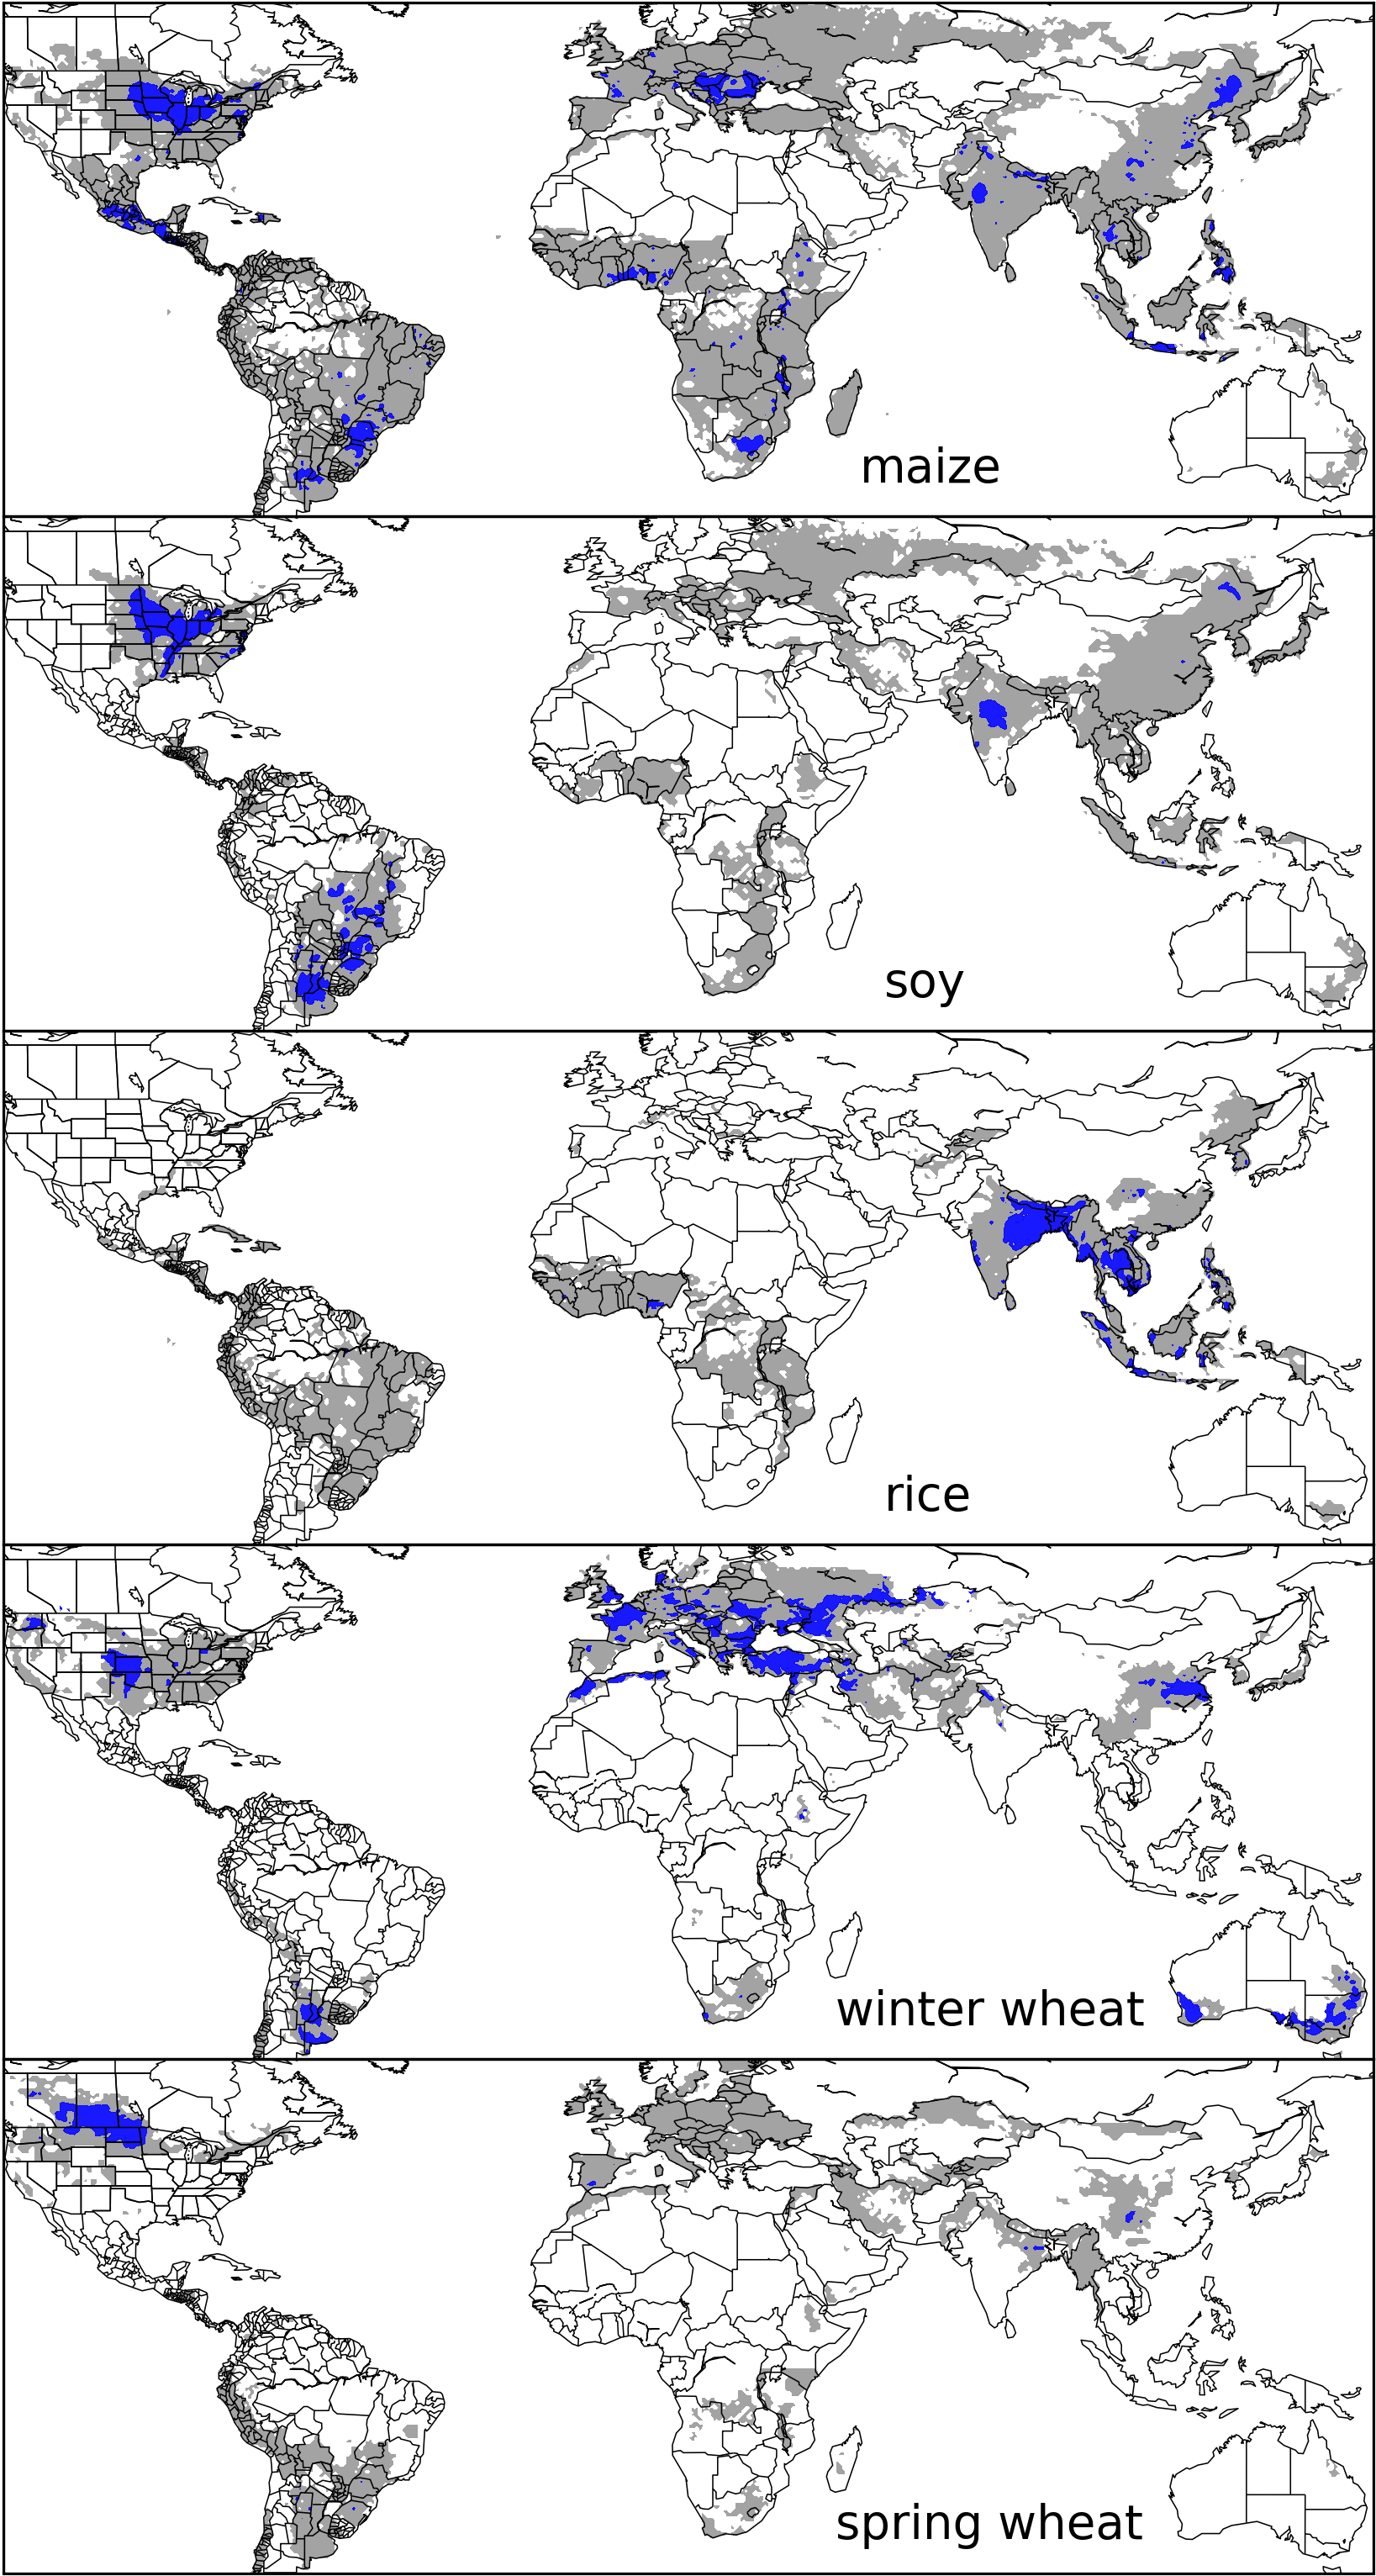
\includegraphics[width=7cm]{figures/croparea.png}
   \caption{Presently cultivated area for rainfed crops. Blue indicates grid cells with more that 20,000 hectares ($\sim$10\% of an equatorial grid cell). 
   Gray contour shows area with more that 10 hectares cultivated. Cultivated areas for maize, rice, and soybean are taken from the MIRCA2000 (``Monthly Irrigated and Rainfed Crop Areas around the year 2000'') dataset \citep{Portmann2010}. 
  Areas for winter and spring wheat areas are adapted from MIRCA2000 and two other sources; see text for details.  For analogous figure of irrigated crops, see Figure \ref{S1}.}
   \label{fig:crop_area}
\end{figure}

The GGCMI Phase I intercomparison was a relatively limited computational exercise, requiring yield simulations for 19 crops across a total of 310 model-years of historical scenarios, and had the participation of 21 modeling groups.
The GGCMI Phase II protocol is substantially larger, involving over 1400 individual 30-year scenarios, or over 42,000 model-years; 12 modeling groups nevertheless participated. To reduce the computational load, the GGCMI Phase II protocol reduced the number crops to 5 (maize, rice, soybean, spring wheat, and winter wheat). 
The reduced set of crops includes the three major global cereals and the major legume and accounts for over 50\% of human calories (in 2016, nearly 3.5 billion tons or 32\% of total global crop production by weight) \citep{FAOSTAT}. This set of major crops has the advantage of  historical yield data at sub-national scale across the globe \citep{Ray2012,iizumi_historical_2014}, and has been frequently used in agricultural analyses \citep[e.g.][]{muller_global_2017,porwollik_spatial_2016}.  % put gratuitous citations here!

The Phase II protocol involves a suite of uniform perturbations from a historical weather scenario. 
The baseline climate scenario for GGCMI Phase II is one of the weather products used in Phase I, daily climate inputs for the years period 1980-2010 from the 0.5 degree NASA AgMERRA (``Agricultural''-modified Modern Era Retrospective analysis for Research and Applications) gridded re-analysis product. AgMERRA is specifically designed for agricultural modeling, with satellite-corrected precipitation \citep{Ruane2015}. 
The experimental protocol consists of 9 levels for precipitation perturbations, 7 for temperature, 4 for [CO$_2$], and 3 for applied nitrogen, for a total of 756 simulations, 672 for rainfed agriculture and additional 84 for irrigated (Table \ref{table:inputs}).  For irrigated simulations, models are set to apply near-perfect irrigation to keeps soils wet throughout the entire growing period, with no limitations in water supply. 
Values of climate variable perturbations are selected to represent reasonable ranges for changes over the medium term (to end of 2100) under business-as-usual emissions. 
The resulting GGCMI Phase II dataset therefore captures the distribution of crop model responses over the space of future potential climate conditions.

\begin{table}[t]
\caption{GGCMI Phase II input parameter levels for each dimension. Temperature and precipitation values indicate the perturbations from the historical climatology. W-percentage does not apply to the irrigated (W$_{inf}$) simulations, which are simulated at the maximum beneficial levels of water. Bold font indicates the `baseline' or historical level for each dimension. Adaptation dimension (A1) repeats all (A0) simulations except the growing season in held fixed. One model provided simulations at the T + 5 level. See Figure S3 in the supplement for number of simulations associated with each combination of input levels.}
\label{table:inputs} 
    \begin{tabular}{lcc} 
        \tophline \vspace{1mm}
        \textbf{Input variable} & \textbf{Simulation input values} & \textbf{Unit} \\ \middlehline \vspace{1mm}
        [CO$_2$] (C) & \textbf{360}, 510, 660, 810 & ppm\\ \middlehline \vspace{1mm}
        Temperature (T) & -1, \textbf{0}, 1, 2, 3, 4, 6 & $^{\circ}$C\\ \middlehline \vspace{1mm}
        Precipitation (W) & -50, -30, -20, -10, \textbf{0}, & \% \\
        {} & 10, 20, 30, (and W$_{inf}$) & {} \\ \middlehline \vspace{1mm}
        Applied nitrogen (N) & 10, 60, \textbf{200} & kg ha$^{-1}$ \\ \middlehline \vspace{1mm}
        Adaptation (A) & \textbf{A0: none}, A1: new cultivar to maintain original growing season length & -\\ \bottomhline
    \end{tabular}\\
\end{table}

While all perturbations are applied uniformly across the historical timeseries, they are applied in different ways. Temperature perturbations are applied as absolute offsets from the daily mean, minimum, and maximum temperature time series for each grid cell.
Precipitation perturbations are applied as fractional changes at the grid cell level. [CO$_2$] and nitrogen levels are specified as discrete values applied uniformly over all grid cells. 
Perturbations are applied independently and the protocol samples over all possible permutations. This choice means that [CO$_2$] changes are applied independently of changes in climate variables, so that higher [CO$_2$] is not associated with particular climate changes, e.g.\ higher temperatures. 

Each model is run at 0.5 degree spatial resolution and covers all currently cultivated areas and much of the uncultivated land area. See Figure \ref{fig:crop_area} for the present-day cultivated area of rainfed crops, provided by the MIRCA2000 (Monthly Irrigated and Rainfed Crop Area) data product \citep{Portmann2010}, and Supplementary Figure S1 for irrigated crops. 
Coverage extends considerably outside currently cultivated areas because cultivation will likely shift under climate change.  
To reduce the computational burden, however, the protocol requires simulation only over \textcolor{blue}{JIM -- XX\%} of Earth surface area.  
Areas are not simulated if they are assumed to remain non-arable even under an extreme climate change; these regions include Greenland, far-northern Canada, Siberia, Antarctica, the Gobi and Sahara Deserts, and central Australia. 
The protocol also eliminates regions judged unsuitable for cropland for non-climatic reasons. 
Selection criterion involve a combination of soil suitability indices at 10 arc-minute resolution and excludes those 0.5 degree grid cells in which at least 90\% of the area is masked as unsuitable according to any single index, and which do not contain any currently cultivated cropland. 
% COMMENTED til we understand (i.e.\ soil quality is not not categorized as "minimal" or "moderate" constraints).and do not contain any cropland  
% CITATION (downloaded from www.gaez.iiasa.ac.at/). 
Soil suitability indices measure excess salt, oxygen availability, rooting conditions, toxicities, and workability, and are provided by the IIASA (International Institute for Applied Systems Analysis) Global Agro-Ecological Zone model \citep[GAEZ, ][]{gaez}. 
The procedure follows that proposed by \citet{pugh_climate_2016}. 
All modeling groups simulate the minimum required coverage, but some provide simulations that extend into masked zones, including e.g.\ the Sahara Desert and Central Australia.

\subsection{Harmonization between models}
The 12 models included in GGCMI Phase II are all process-based crop models that are widely used in impacts assessments (Table \ref{table:models}).
Although some models share a common base (e.g.\ the LPJ family or the EPIC family of models), they have subsequently developed independently.  Wherever possible, the GGCMI Phase II protocol harmonizes inputs, but
differences in model structure mean that several key factors cannot be fully standardized across the experiment. These include soil treatment (which affects soil organic matter and carry-over effects of soil moisture across growing years) and baseline climate inputs.  

%Not all modeling teams provide the full simulation protocol, for instance, CARIAB and JULES do not simulate the nitrogen dimension and some crops are not parameterized in each model (see Table \ref{table:models} for details). 

While 10 of the 12 models participating in GGCMI Phase II use the AgMERRA historical daily climate data product, two models require sub-daily input data and thus use different baseline climate inputs:
PROMET uses the ERA-Interim reanalysis \citep{dee2011era}; JULES uses a bias-corrected version of ERA-Interim, the 3-hour WFDEI (WATCH-Forcing-Data-ERA-Interim) \citep{weedon2014wfdei}, selecting the WFDEI version in which precipitation is bias-corrected against the CRU TS3.101/TS3.21 precipitation totals\citep{harris_cru_2014}.
The WFDEI data product differs slightly, ERA-Interim more pronounced from  AgMERRA. Figures \ref{SXX} and \ref{SXX} show temperature and precipitation in the three data products over currently cultivated areas for XX and XX crops. At this aggregation level, temperatures are very similar between data products, ERA-Interim being about 1.0 and 0.3$\circ$C cooler in rice and maize growing areas, respectively. For precipitation, ERA-Interim is substantially wetter in wheat areas (+60mm year$^{-1}$) and also in some years for rice, maize and soybean areas.
%There are some larger differences for ERA-Interim, especially for rice area air temperatures, which are roughly 1K lower and for wheat and maize precipitation (Figures Sxx and Syy).
%---- NOTE-- XX EJM - doesn't make sense that ERA-Interim differs in temperature from WFDEI since above you said the only different was precipitation
% WFDEI is a bias-corrected version of ERA-Interim -- in all variables. Hopefully more clear now.
These differences are still relatively small compared to the perturbations tested in the protocol.

%\textcolor{red}{Explain what WFDEI does and how it's constructed. Then a sentence about differences in temp and precip absolutes and variability between these datasets.? Did you check how much this matters to yields? Are you assuming that baseline doesn't matter and you'll still capture changes well?}
Planting dates and growing season lengths are standardized across models, following the procedure described in \citet{Elliott2015} for the \textit{fullharm} setting. In contrast to GGCMI Phase I \citep{Elliott2015}, we here assume identical growing seasons for rainfed and irrigated scenarios, to allow for direct comparability of simulations along the W dimension, in which irrigation (\textit{W$_{inf}$}) is one element (see Table \ref{table:inputs}). 
While sowing dates are prescribed directly in models, the length of the growing season is a product of crop phenology, which in turn is mostly driven by phenological parameters and temperature. Modelers are asked to adjust the phenological parameters so that growing season length on average matches the harmonization target. Given that temperature varies between years, individual years can vary from the harmonization target.
Harmonization of growing seasons is crop- and location-specific, i.e. they vary in space and per crop but not across models. 
For example, at present maize is sown in March in Spain, in July in Indonesia, and in December in Namibia \citep{Portmann2010}.
One exception is CARAIB, which did not harmonize against provided growing season data \citep{Elliott2015}, but kept their own growing seasons.
 
%\textcolor{red}{sounds like... Growing seasons are specified in terms of climatological variables, and so the actual length of crop growth alters under climate change. XX need more here.} 
To roughly account for the importance of adaptation in agricultural production, the GGCMI Phase II protocol includes two sets of experiments that sample adaptation. 
As simulated growing seasons respond to temperatures, these are sensitive to changes along the T dimension in the CTWN experiment. For adaptation, a fifth dimension ``A'' was added, for adaptation in phenological traits.
The first set (``A0'', where 0 denotes ``no adaptation'') involves growing seasons with unmodified, harmonized phenological parameters, which generally result in shorter growing seasons in warmer scenarios. 
The second set, (``A1'', with adaptation) holds the length of the growing season fixed at that of the baseline climate scenario. 
For this, modelers had to repeat the baseline calibration of growing seasons length at all temperature levels along the T dimension (Table \ref{table:inputs}).
Even though CARAIB did not harmonize the growing seasons to GGCMI targest, their ``A1'' simulations follow the same principle, so that phenological parameters are modified to keep growing seasons roughly constant across different warming scenarios.
These ``A1'' simulations roughly capture the case in which adaptive crop cultivar choice maintain the growing season length so that crops reach maturity at roughly the same time as do current varieties under the current temperature regime. 
This assumption is simplistic, and does not reflect realistic opportunities and limitations to adaptation \citep{vadez2012adaptation,challinor2018improving}, but provides some insight into how crop modifications could alter projected impacts on yields.

Growing seasons for maize, rice, and soybean are taken from the SAGE (Center for Sustainability and the Global Environment, University of Wisconsin) crop calendar \citep{Sacks2010} and are identical to those used in GGCMI Phase I \citep{Elliott2015}.
In GGCMI Phase II, we separately treat spring and winter wheat and so must define different growing seasons for each.
We use the SAGE crop calendar, which separately specifies spring and winter wheat, as the primary source for \textcolor{blue}{JIM -- XX\% of grid cells}. 
In the remaining areas where no SAGE information is available, we turn to, in order of preference, the MIRCA2000 crop calendar \citep{Portmann2010} and to simulated LPJmL growing seasons \citep{waha2012climate}.  
These datasets each provide several options for wheat growing season for each grid cell, but do not label them as spring or winter wheat. We assign a growing season to each wheat type for each location based on its baseline climate conditions. 
A growing seasons is assigned to winter wheat if all of the following hold:
% below requires \usepackage{enumitem}
\begin{itemize} %[noitemsep]
\item the monthly mean temperature is below freezing point (<0$^\circ$C) at most for 5 months per year (i.e. winter is not too long)
\item the coldest 3 months of a year are below 10$^\circ$C (i.e. there is a winter)
\item the season start date fits the criteria that
  \begin{itemize} 
    \item if in the N.\ hemisphere, it is after the warmest \textit{or} before the coldest month of the year (as winter is around the end/beginning of the calendar year)
    \item if in the S.\ hemisphere, it is after the warmest \textit{and} before the coldest month of the year (as winter is in the middle of the calendar year)
    \end{itemize}
\end{itemize}
and to spring wheat otherwise. 
%\textcolor{red}{does the mean monthly T criterion relate to the grid cell climatology over the whole year or to the grid cell climatology only during the growing season? also, why is there a N./S. hemisphere difference?}
% it's the monthly mean temperature not the mean monthly temperature. corrected. Winter is in the middle of the calendar year in the S. hemisphere, so this "before" and "after" criterion needs to change.

Nitrogen application is also standardized in timing across models. 
N fertilizer is applied in two doses, as is often the norm in actual practice, to reduce losses to the environment. 
In the GGCMI Phase II protocol, half of the total fertilizer input is applied at sowing and the other half on day 40 after sowing, for all crops except for winter wheat. 
For winter wheat, in practice the application date for the second N fertilizer application varies according to local temperature, because the length of winter dormancy can vary strongly. 
In the GGCMI Phase II protocol, the second fertilization date for winter wheat is set to the middle day of the first month after sowing that has average temperatures above 5$^\circ$C, with hard limits between 40 days from planting and 50 from maturity.
%\textcolor{red}{What if these criteria disagree with each other? do you take the 50 day / 40 day limit and violate the first criterion?}

All stresses are disabled in models other than those related to nitrogen, temperature, and water. 
For example, model responses to alkalinity, salinity, and non-nitrogen nutrients are all disabled. 
For a better controlled experiment, no other external N inputs are permitted -- that is, there is no atmospheric deposition of nitrogen --  but some models allow additional release of plant-available nitrogen through mineralization in soils. 
Soil mineralization is a part of model treatments of soil organic matter and cannot be disabled in some models (e.g. LPJmL, LPJ-GUESS). 
Some additional differences in model structure mean that several key factors are not standardized across the experiment. 
For example, carry-over effects across growing years including residue management and soil moisture are treated differently across models.

\subsection{Output data products}
All models in GGCMI Phase II provide 7 mandatory output variables (Table \ref{table:outputs}, bold), if available. 
For each scenario, 0.5 degree grid cell and crop, models provide 30-year timeseries of annual crop yields in units of tons ha$^{-1}$ year$^{-1}$, as well as total aboveground biomass yield; the dates of planting, anthesis, and maturity; applied irrigation water in irrigated scenarios; and total evapotranspirtation. 
(Note that several of the EPIC-family models do not output the anthesis date.)
Besides these mandatory 7 data products, the protocol requests any or all of 18 optional additional output variables (Table \ref{table:outputs}, plain text).
Participating modeling groups provided between 3 (PEPIC) and 18 (APSIM-UGOE) of these optional variables. 
%Finally, some models provide additional variables not specified in the protocol, such as more detailed separation of total nitrogen losses which were supplied by LPJmL, LPJ-GUESS and pDSSAT.

\begin{table}[]
\caption{Output variables requested per crop in the GGCMI Phase II protocol. Items in \textbf{bold} are mandatory, if available in that model.}
\label{table:outputs}
\begin{tabular}{lll}
        \tophline \vspace{1mm}
Variable                                & variable name             & units \\
\middlehline \vspace{1mm}
\textbf{Yield}                                   & \textbf{yield\_<crop>}     & \textbf{t ha$^{-1}$ yr$^{-1}$ (dry matter)}\\
\textbf{Total above ground biomass yield}        & \textbf{biom\_<crop>}      & \textbf{t ha$^{-1}$ yr$^{-1}$ (dry matter)}\\
\textbf{Actual planting date}                    & \textbf{plant-day\_<crop>} & \textbf{day of year}\\
\textbf{Anthesis date}                           & \textbf{anth-day\_<crop>}  & \textbf{days from planting} \\
\textbf{Maturity date}                           & \textbf{maty-day\_<crop>}  & \textbf{days from planting}\\
\textbf{Applied irrigation water}                & \textbf{pirrww\_<crop>}    & \textbf{mm yr$^{-1}$} \\
\textbf{Evapotranspiration (growing season sum)} & \textbf{etransp\_<crop>}   & \textbf{mm yr$^{-1}$ (firr scenarios only)}\\ \middlehline
Transpiration (growing season sum)                       & transp\_<crop>    & mm yr$^{-1}$ \\
Evaporation (growing season sum)                         & evap\_<crop>      & mm yr$^{-1}$ \\
Runoff (total growing season sum, subsurface + surface)  & runoff\_<crop>    & mm yr$^{-1}$                    \\
Total available soil moisture in root zone *             & trzpah2o\_<crop>  & mm yr$^{-1}$                    \\
Total root biomass                                       & rootm\_<crop>     & t ha$^{-1}$ yr$^{-1}$ (dry matter)  \\
Total Nr uptake (total growing season sum)               & tnrup\_<crop>     & kg ha$^{-1}$ yr$^{-1}$              \\
Total Nr inputs (total growing season sum)               & tnrin\_<crop>     & kg ha$^{-1}$ yr$^{-1}$              \\
Total Nr losses (total growing season sum)               & tnrloss\_<crop>   & kg ha$^{-1}$ yr$^{-1}$              \\
Gross primary production (GPP)                           & gpp\_<crop>       & gC m$^{-2}$ yr$^{-1}$               \\
Net primary production (NPP)                             & npp\_<crop>       & gC m$^{-2}$ yr$^{-1}$               \\
CO$_2$ response scaler on NPP                            & co2npp\_<crop>    & - \{0..inf\}                \\
water response scaler on NPP                             & h2onpp\_<crop>    & - \{0..1\}                  \\
temperature response scaler on NPP                       & tnpp\_<crop>      & - \{0..1\}                  \\
Nr response scaler on NPP                                & nrnpp\_<crop>     & - \{0..1\}                  \\
Other nutrient response scaler on NPP                    & ornpp\_<crop>     & - \{0..1\}                  \\
CO$_2$ response scaler on transpiration                  & co2trans\_<crop>  & - \{0..1\}                  \\
maximum stress response scaler                           & maxstress\_<crop> & - \{0..1\}                  \\
Maximum LAI                                              & laimax\_<crop>    & m$^{2}$ m$^{-2}$           \\        
\bottomhline
* growing season sum, basis for computing average soil moisture & {} & {} \\
\end{tabular}
\end{table}

All output data is supplied as netCDF version 4 files, each containing values for one variable in a 30-year timeseries associated with a single scenario, for all grid cells. Filenames follow the naming conventions of GGCMI Phase I \citep{Elliott2015}, which themselves are taken from those of ISIMIP \citep{frieler2017assessing}. File names are specified (in small caps) as 

$[model]\_[climate]\_hist\_fullharm\_[irrig.scenario]\_[variable]\_[crop]\_global\_annual\_[start-year]\_[end-year].nc4$

\noindent Here $[model]$ is the crop model name; $[climate]$ is the original climate input data set (typically AgMERRA); $[irrig.scenario]$ is the irrigation setting ("firr" for fully irrigated and "noirr" for fully rainfed); $[variable]$ is the output variable (of those in Table \ref{table:outputs}); $[crop]$ is the crop abbreviation ("mai" for maize, "ric" for rice, "soy" for soybean, "swh" for spring wheat, and "wwh" for winter wheat); and $[start-year]$ and $\_[end-year]$ specify the first and last years recorded on file.
All filenames include the identifier $global$ to distinguish them as global model output.

Output data is provided on a regular geographic grid, identical for all models. 
Grid cell centers span latitudes -89.75 to 89.75$^{\circ}$ and longitudes from -179.75 to 179.75$^{\circ}$. 
Missing values  where no crop growth has been simulated are distinguished from crop failures: a crop failure is reported as zero yield but non-simulated areas (including ocean grid cells) have yields reported as 1.e+20. 
Following NetCDF standards, latitude, longitude and time are included as separate variables in ascending order, with
units "degrees north", "degrees east", and "growing seasons since 1980-01-01 00:00:00". 

% ---- XX well-edited up to here, only lightly below  -----------------
% \textcolor{red}{Clarify this paragraph.} % clear to me?
Following GGCMI Phase I standards, the first entry in the file is the result of the first simulated cropping cycle that is entirely within the given climate input. 
For AgMERRA, where the first year provided is 1980, the first harvest record is thus of 1980, when the prescribed sowing and harvest dates are in 1980 (e.g. sowing in March and harvest in September 1980) but is of 1981 if sowing is later in a calendar year than harvest (e.g. sowing in September 1980 and harvest in March 1981). 
To avoid distortions in harvest events, output files report the sequence of growing periods rather than calendar years. 
In most cases, this is equivalent, as there is always only one sowing event per calendar year.
As harvest events are internally determined as a function of mostly temperature, these can vary between individual years. 
If harvest events are around the end of the calendar year (Dec. 31), reported values could contain 2 (one in early January and one in late December), 1 (normal) or none (last was in December of previous year and next is in January of the following year) harvest event if reported per calendar year.
As such, the time dimension in the netCDF files is not on calendar years, but on "growing seasons" (sée above).

\section{Models contributing}
\label{S:3}
\begin{table*}[t]
\caption{Models included in GGCMI Phase II and the number of C, T, W, and N simulations that each performs, with 756 as the maximum for A0 (no adaptation) and 648 as the maximum for A1 (maintaining growing season adaptation; in A1, T0 is skipped as there is no adaptation to temperature-driven shortening of growing seasons there). 
``N-Dim.'' indicates whether the simulations include varying nitrogen levels. Two models provide only one nitrogen level. 
All models provide the same set of simulations across all modeled crops, but some omit individual crops. (For example, APSIM does not simulate winter wheat.)}
\label{table:models}
  \begin{tabular}{p{6cm} p{1cm} p{1cm} p{1cm} p{1cm} p{1cm} p{1cm} p{1.9cm}}
        \tophline
    {\textbf{Model (Key Citations)}}&{\textbf{Maize}}&{\textbf{Soybean}}&{\textbf{Rice}}&{\textbf{Winter wheat}}&{\textbf{Spring wheat}}&{\textbf{N dim.}}&{\textbf{Sims per crop (A0 / A1)}}\\ \middlehline
        {\textbf{APSIM-UGOE},   \citet{KEATING2003267, HOLZWORTH2014327}} & {X} & {X} & {X} & {--} & {X} & {X} & {44 / 36}\\ \middlehline
        {\textbf{CARAIB},       \citet{Dury2011, Pirttioja2015}} & {X} & {X} & {X} & {X} & {X} & {--} & {\textbf{252 / 216}}\\ \middlehline
        {\textbf{EPIC-IIASA},   \citet{BALKOVIC2014}} & {X} & {X} & {X} & {X} & {X} & {X} & {39 / 0}\\  \middlehline
        {\textbf{EPIC-TAMU},    \citet{Izaurralde06}} & {X} & {X} & {X} & {X} & {X} & {X} & {\textbf{756 / 648}}\\ \middlehline
        {\textbf{JULES},        \citet{Osborne2015, Williams2015, Williams2017}} & {X} & {X} & {X} & {--} & {X} & {--} & {\textbf{252 / 0}}\\ \middlehline
        {\textbf{GEPIC},        \citet{LIU2007478, FOLBERTH201221}} & {X} & {X} & {X} & {X} & {X} & {X} & {430 / 181}\\ \middlehline
        {\textbf{LPJ-GUESS},    \citet{Lindeskog2013, Olin2015}} & {X} & {--} & {--} & {X} & {X} & {X} & {\textbf{756 / 648}}\\  \middlehline
        {\textbf{LPJmL},        \citet{von_Bloh_implementing_2018}} & {X} & {X} & {X} & {X} & {X} & {X} & {\textbf{756 / 648}}\\ \middlehline
        {\textbf{ORCHIDEE-crop},\citet{Wu2016}} & {X} & {--} & {X} & {X} & {--} & {X} & {33 / 0}\\ \middlehline
        {\textbf{pDSSAT},       \citet{Elliott2014b, JONES2003235}} & {X} & {X} & {X} & {X} & {X} & {X} & {\textbf{756 / 756}}\\ \middlehline
        {\textbf{PEPIC},        \citet{LIU2016164, LIU2016}} & {X} & {X} & {X} & {X} & {X} & {X} & {149 / 121}\\ \middlehline
        {\textbf{PROMET},       \citet{Hank2015, MAUSER2015}} & {X} & {X} & {X} & {X} & {X} & {X} & {261 / 232}\\ \middlehline
        {Totals} & {12} & {10} & {11} & {11} & {11} & {10} & {5240 | 3378}\\
        \bottomhline
    \end{tabular}
\end{table*}

The contributions of the 12 crop models supplying data to the GGCMI Phase II archive are described in Table \ref{table:models}.
Modeling groups did not all implement the full protocol described above. Given the substantial computational requirements, different participation tiers were specified to allow submission of smaller sub-sets of the full protocol. 
These subsets were designed as alternate samples across the 4 dimensions of the CTWN space,with \textit{full} (12) and \textit{low} (4) options for the C $\times$ N variables, and \textit{full} (63), \textit{reduced} (31), and \textit{minimum} (9) options for T $\times$ W variables (described below). All participating modeling groups provided identical coverage of the CTWN parameter space for different crops, but some provided no or a more limited sample for scenarios with adaptation (A1).
This is, as the adaptation dimension is deemed a side-aspect of the GGCMI Phase II experiment that is only analyzed in specific applications.
The different participation levels are defined by combining the CxN sets with the TxW sets:
\begin{itemize}
\item{\textbf{full}: all 756 A0 simulations (all 12 CxN * all 63 TxW)}
\item{\textbf{high}: 362 simulations (all 12 CxN combinations * \textit{reduced} TxW set of 31 combinations)}
\item{\textbf{mid}: 124 simulations (\textit{low} 4 CxN combinations * \textit{reduced} TxW set of 31 combinations)}
\item{\textbf{low}: 36 simulations (\textit{low} 4 CxN combinations * \textit{minimum} TxW set of 9 combinations)}
\end{itemize}
%\textcolor{red}{Why are the A1 simulations only 658 in total? pDSSAT has 756 in the A1 folder}
% For A1, T0 sims are identical with A0 -- there is no adaptation to shorter growing seasons if they don't get shorter. Added that to table caption

Of the 12 models submitting data, 6 followed the \textit{full} protocol; these are marked with italic text in Table \ref{table:models}. However, note that two of these models (CARAIB and JULES) intrinsically cannot represent nitrogen effects and so do not sample over the the nitrogen dimension at all. 2 models followed \textit{high} with minor modifications (GEPIC adding an additional T level and PROMET omitting the intermediate N level). 1 model (PEPIC) followed \textit{mid} but included an additional C level. 3 models approximately followed \textit{low} with APSIM-UGOE and EPIC-IIASA providing some additional levels and ORCHIDEE-crop omitting a TxW combination.  

The combinations of perturbation values in the CxN and TxW parameter spaces used in the various participation levels are chosen to provide maximum coverage over plausible future values. For the CxN space, we specify:
\begin{itemize}
\item \textit{full} as 12 pairs, with 4 C values (360, 660, 810 ppm) and 3 N (10, 60, 200 kg ha$^{-1}$ yr$^{-1}$ ))
\item \textit{low} as only 4 pairs: C360\_N10, C360\_N200, C660\_N60, C810\_N200) 
\end{itemize}
    
For the TxW space we specify:
\begin{itemize}
\item \textit{full} as all 7 T levels and 9W levels.
\item \textit{reduced} as 31 alternating combinations, with different Ws for even Ts than for odd Ts. For even Ts (i.e.\ T0,T2,T4,T6), we use W = -50,-20,0,+30 = 4$\cdot$4 = 16 pairs. For odd Ts (i.e.\ T-1,T1,T3) , we use W = -30, -10, +10, +30, inf = 3$\cdot$5 = 15 pairs.
\item \textit{minimum} as 9 combinations: T-1W-10, T0W10, T1W-30, T2W-50, T2W20, T3W30, T4W0, T4Winf, T6W-20
\end{itemize}

%%%%%%%%%%%%%%%%%%%%%%%%%%%%%%%%%%%%%%%%%%%%%%%%%%%%%%%%%%%%%%%
%%%%%%%%%%%%%%%%%%%%%%%%%%%%%%%%%%%%%%%%%%%%%%%%%%%%%%%%%%%%%%%
%%%%%%%%%%%%%%%%%%%%%%%%%%%%%%%%%%%%%%%%%%%%%%%%%%%%%%%%%%%%%%%
\section{Results}
\label{S:4}

To illustrate the properties of the GGCMI Phase II model simulations, we provide both an assessment of model performance by comparing to observed yields, and selected case studies showing the spread of model responses to climate and management inputs.

\subsection{Assessment of model performance}
\begin{figure*}[ht]
    \centering
    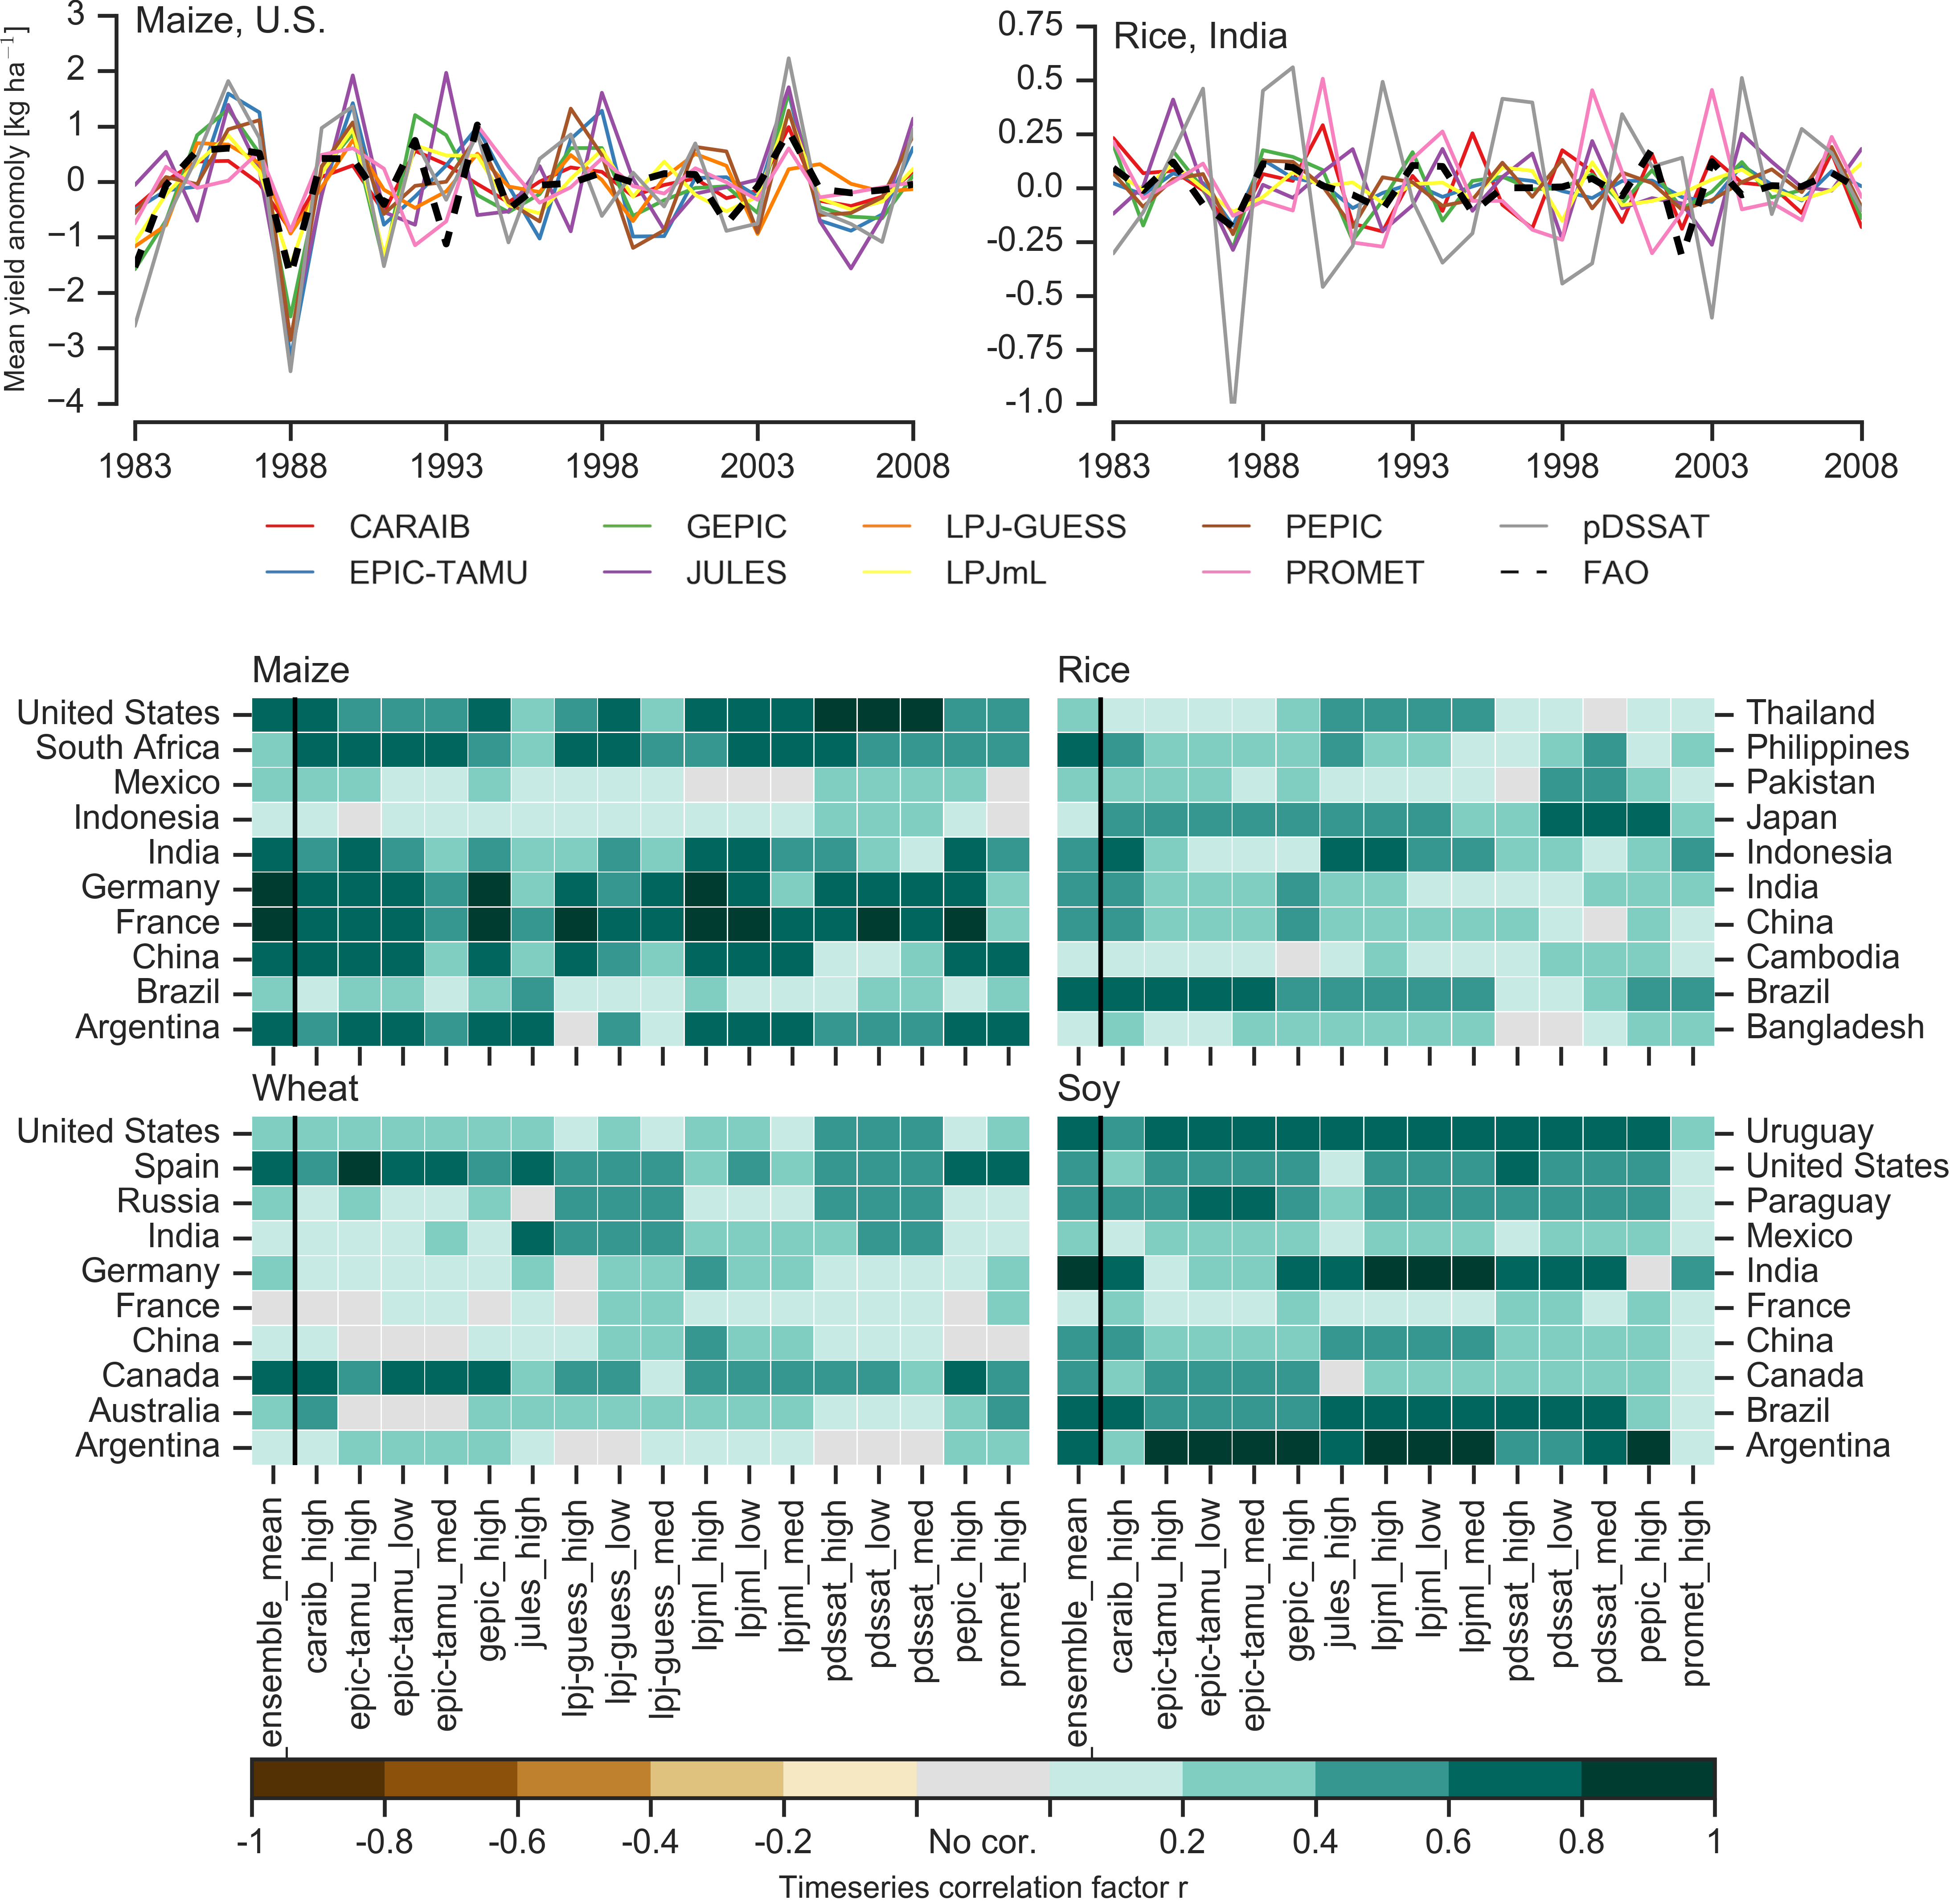
\includegraphics[width=14cm]{figures/Agformet_validation.png}
    \caption{Assessment of crop model performance in GGCMI Phase II, following protocol of GGCMI Phase I \citep{muller_global_2017}. 
    \textbf{Top:} example time series comparison between simulated crop yield and FAO data \citep{FAOSTAT} at the country level for two example cases: US maize (a good case), and rice in India (mixed case), both for the high nitrogen application level. 
    \textbf{Bottom:} the heatmaps illustrate the Pearson $r$ correlation coefficient between the detrended simulation mean yield at the country level compared to the detrended FAO yield data for the top producing countries for each crop with continuous FAO data over the 1981-2010 period. 
    Models that provided different nitrogen application levels are shown with low (10 kg N ha$^{-1}$), med (60 kg N ha$^{-1}$), and high (200 kg N ha$^{-1}$) label (models that did not simulate different nitrogen levels are analogous to a high nitrogen application level). 
    The ensemble mean yield, show in the leftmost column, is also correlated with the FAO data (not the mean of the correlations). 
    Wheat contains both spring wheat and winter wheat simulations where supplied, else one or the other (see Table \ref{table:models} ). 
    Differences by region and crop are stronger than difference between models, e.g.\ horizontal bars are more similar in color than vertical bars.}
    \label{fig:simulation_val}
\end{figure*}

Evaluating the performance of crop models in the GGCMI Phase II archive is complicated by the artificial nature of the protocol: the settings in the CTWN-A experiment design do not reflect actual conditions in the real world. 
The protocol includes one scenario of near-historical climate inputs (T$_0$, W$_0$, C$_360$), but the prescribed uniform nitrogen application levels do not reflect real-world fertilizer practices. Models also omit detailed calibrations to reflect the performance of historical cultivars. 

We provide a partial evaluation of the models' skill in reproducing crop yield characteristics using the methodology of \citet{muller_global_2017}, who described model characteristics in GGCMI Phase I. 
\citet{muller_global_2017} evaluate how well model crop yield responses in historical run capture real-world yield variations driven by year-to-year temperature and precipitation variations. 
Following this approach, we compare yields in the GGCMI Phase II baseline run with detrended historical yields from the UN Food and Agriculture Organization (FAO) \citep{FAOSTAT} by calculating the Pearson product moment correlation coefficient. 
The procedure is sensitive to the detrending method and the area mask used to aggregate yields; we use a 5-year running mean removal and the MIRCA2000 cultivation area mask for aggregation. 
In some cases the model time series are shifted by one year to account for errors in FAO or model year reporting. 
% XX -- save for later ---- The procedure offers no means of assessing [CO$_2$] fertilization, since [CO$_2$] has been relatively constant over the historical data collection period. 
Because the GGCMI Phase II protocol imposes fixed, uniform nitrogen application levels that are not realistic for individual countries, we evaluate control runs for each model and at multiple N levels in some cases. Nine of the GGCMI Phase II models provide historical runs for all three nitrogen levels (10, 60, and. 200 kg ha$^-1$ yr$^-1$). 

%In order to illustrate the data structure and general features of the ensemble, we show selected results in different aggregation levels (maps, regional aggregations). 
%We focus on yield data, as this dataset if presumably of greatest interest and yield data are the more important and best evaluated outputs of GGCMs.

As expected, correlation coefficients are slightly lower than those found in the GGCMI Phase I evaluation, but models show reasonable fidelity at capturing year-over-year variation (Figure \ref{fig:simulation_val}). 
\textcolor{blue}{JIM -- give a few numbers here}
(Compare to \citet{muller_global_2017} Figures 1--4 and 6.)  
In GGCMI Phase II, as in Phase I, differences in fidelity between regions and crops exceed differences between models: 
that is, Figure \ref{fig:simulation_val} shows more color similarity in horizontal than vertical bars. 
For example, maize in the United States is consistently well-simulated while maize in Indonesia is problematic (mean Pearson correlation coefficients of 0.68 and 0.18, respectively). 
Note that in this methodology, simulations of crops with low year-to-year variability such as irrigated rice and wheat will tend to score more poorly than those with higher variability.
In some cases, especially in the developing world, low correlation coefficients may indicate not model failure but problems in FAO yield data \citep{Ray2012, muller_global_2017}. 
No single model consistently exhibits greater fidelity than others. 
Instead, each model shows near best-in-class performance for at least one location-crop combination. For example for maize pDSSAT is the best model in the US, LPJmL and GEPIC are the best in Germany, PROMET is best in Argentina, PEPIC and LPJ-GUESS are the best in France, and CARAIB is near best in class in South Africa. 

%In general, correlation coefficients in GGCMI Phase II are slightly below those of Phase I, likely because of unrealistic nitrogen levels, lack of country level calibration in some models, and restriction to only the MICRA aggregation mask used in the comparison in this study. 
%Additionally, the time period used in this case is slightly different from the time period used in \citet{muller_global_2017}. 

\subsection{Model crop yield responses under CTWN forcing}
\begin{figure*}[ht]
\centering
   \includegraphics[width=16.5cm]{figures/baselinecomp_yield_3.png} 
  \caption{Illustration of the spatial pattern of potential yields (left) and yield changes (right) in the GGCMI Phase II ensemble, for three major crops: maize, soybean and rice. Left column (a) shows multi-model mean climatological potential yields for the baseline scenario for (top--bottom) rainfed maize, soybean, and rice. 
   Wheat shows a qualitatively similar response, see Figure S16 in the supplemental material. % XX need dynamic references
   White stippling indicates areas where these crops are not currently cultivated. 
   Absence of cultivation aligns well with the lowest yield contour (0-2 ton ha$^{-1}$). 
   Right column (b) shows the multi-model mean fractional yield change in the T+4 $^{\circ}$C scenario.
 Because yields vary geographically, we show change from a baseline, which we take as the scenario with historical climatology (i.e.\ T and P changes of 0), C of 360 ppm, and applied N at 200 kg N ha$^{-1}$. In T+4 only temperature is changed and other inputs remain fixed at baseline values. 
   Areas without hatching or stippling are those where confidence in projections is high: the multi-model mean fractional change exceeds two standard deviations of the ensemble ($\Delta > 2\sigma$). 
   Hatching indicates areas of low confidence ($\Delta < 1 \sigma$), and stippling areas of medium confidence ($1 \sigma < \Delta < 2 \sigma$). 
   Crop model results in cold areas, where yield impacts are on average positive, also have the highest uncertainty.}
   \label{fig:maizesoybaseline}
\end{figure*}

\begin{figure}[ht]
\centering
   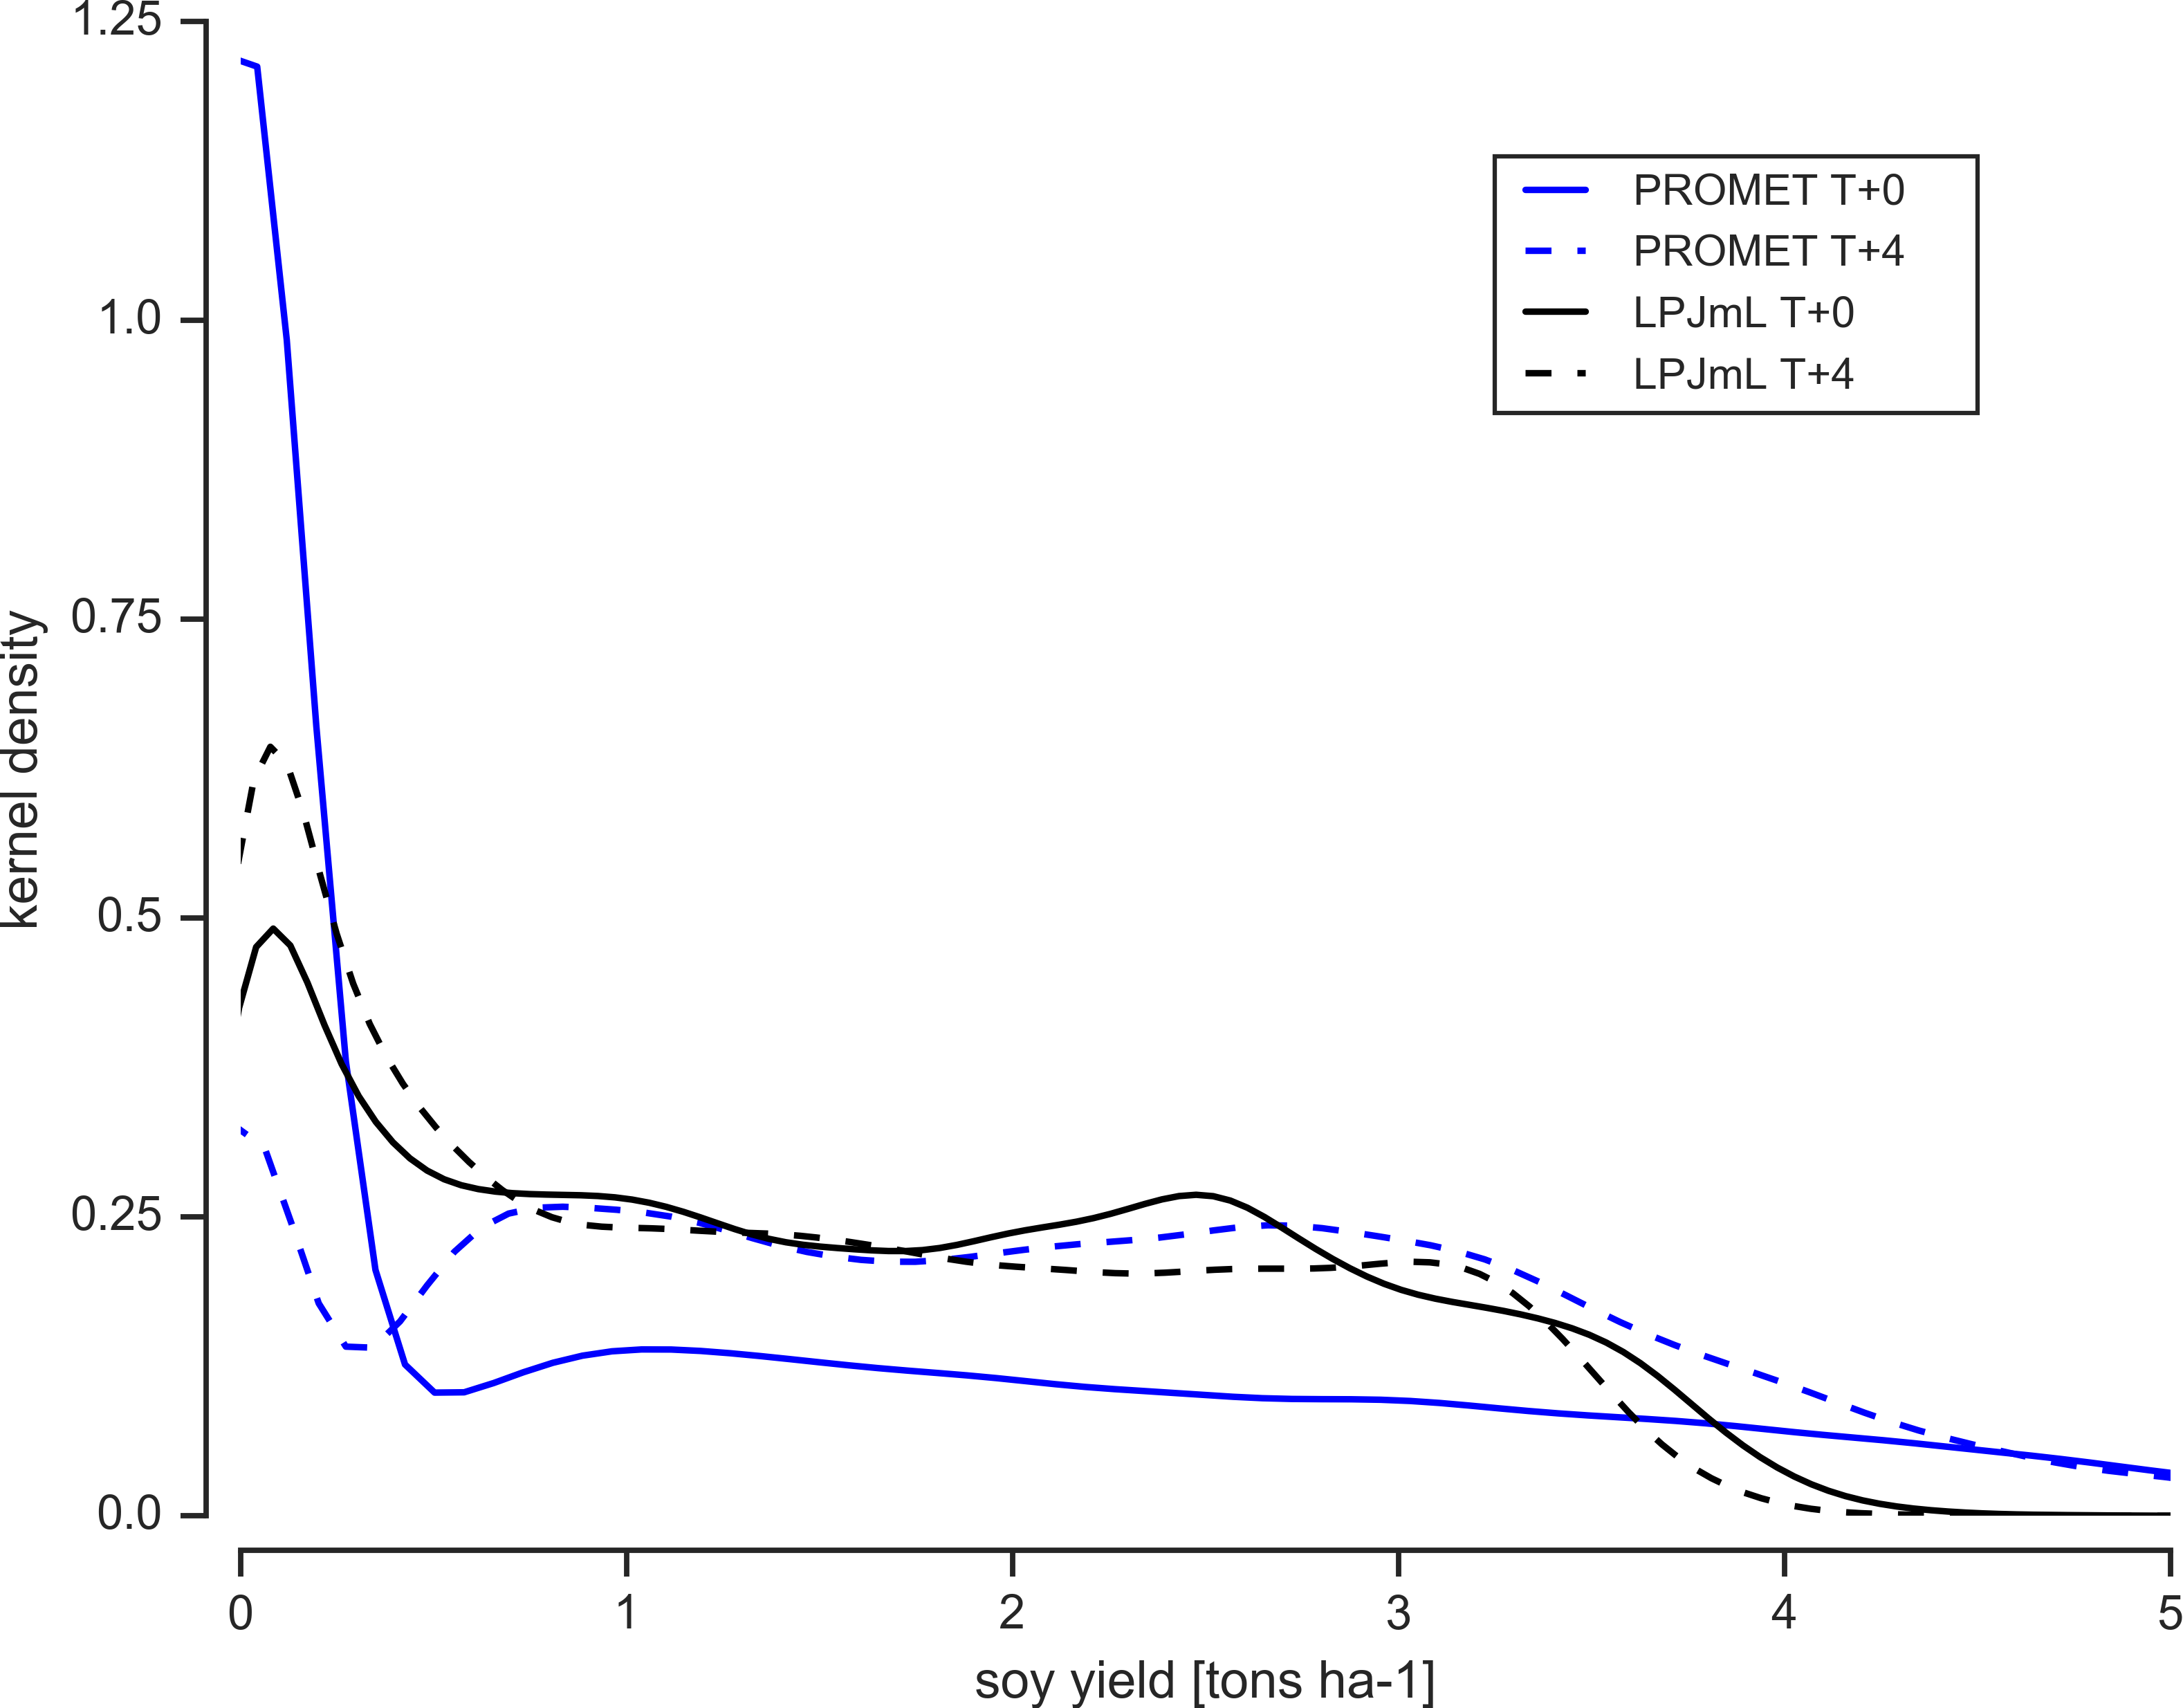
\includegraphics[width=8.3cm]{figures/testhighlatskde.png}
\caption{Kernel density estimate of soybean yields north of 45$^o$ latitude for the PROMET and LPJmL models. Solid lines show the historical climatology and dashed lines show the T+4 (K) case. Note strong reduction in the lowest bin for the T+4 case for PROMET that is spread almost equally over the rest of the distribution.}
\label{fig:highlat}
\end{figure}

\begin{figure*}[ht]
\centering
   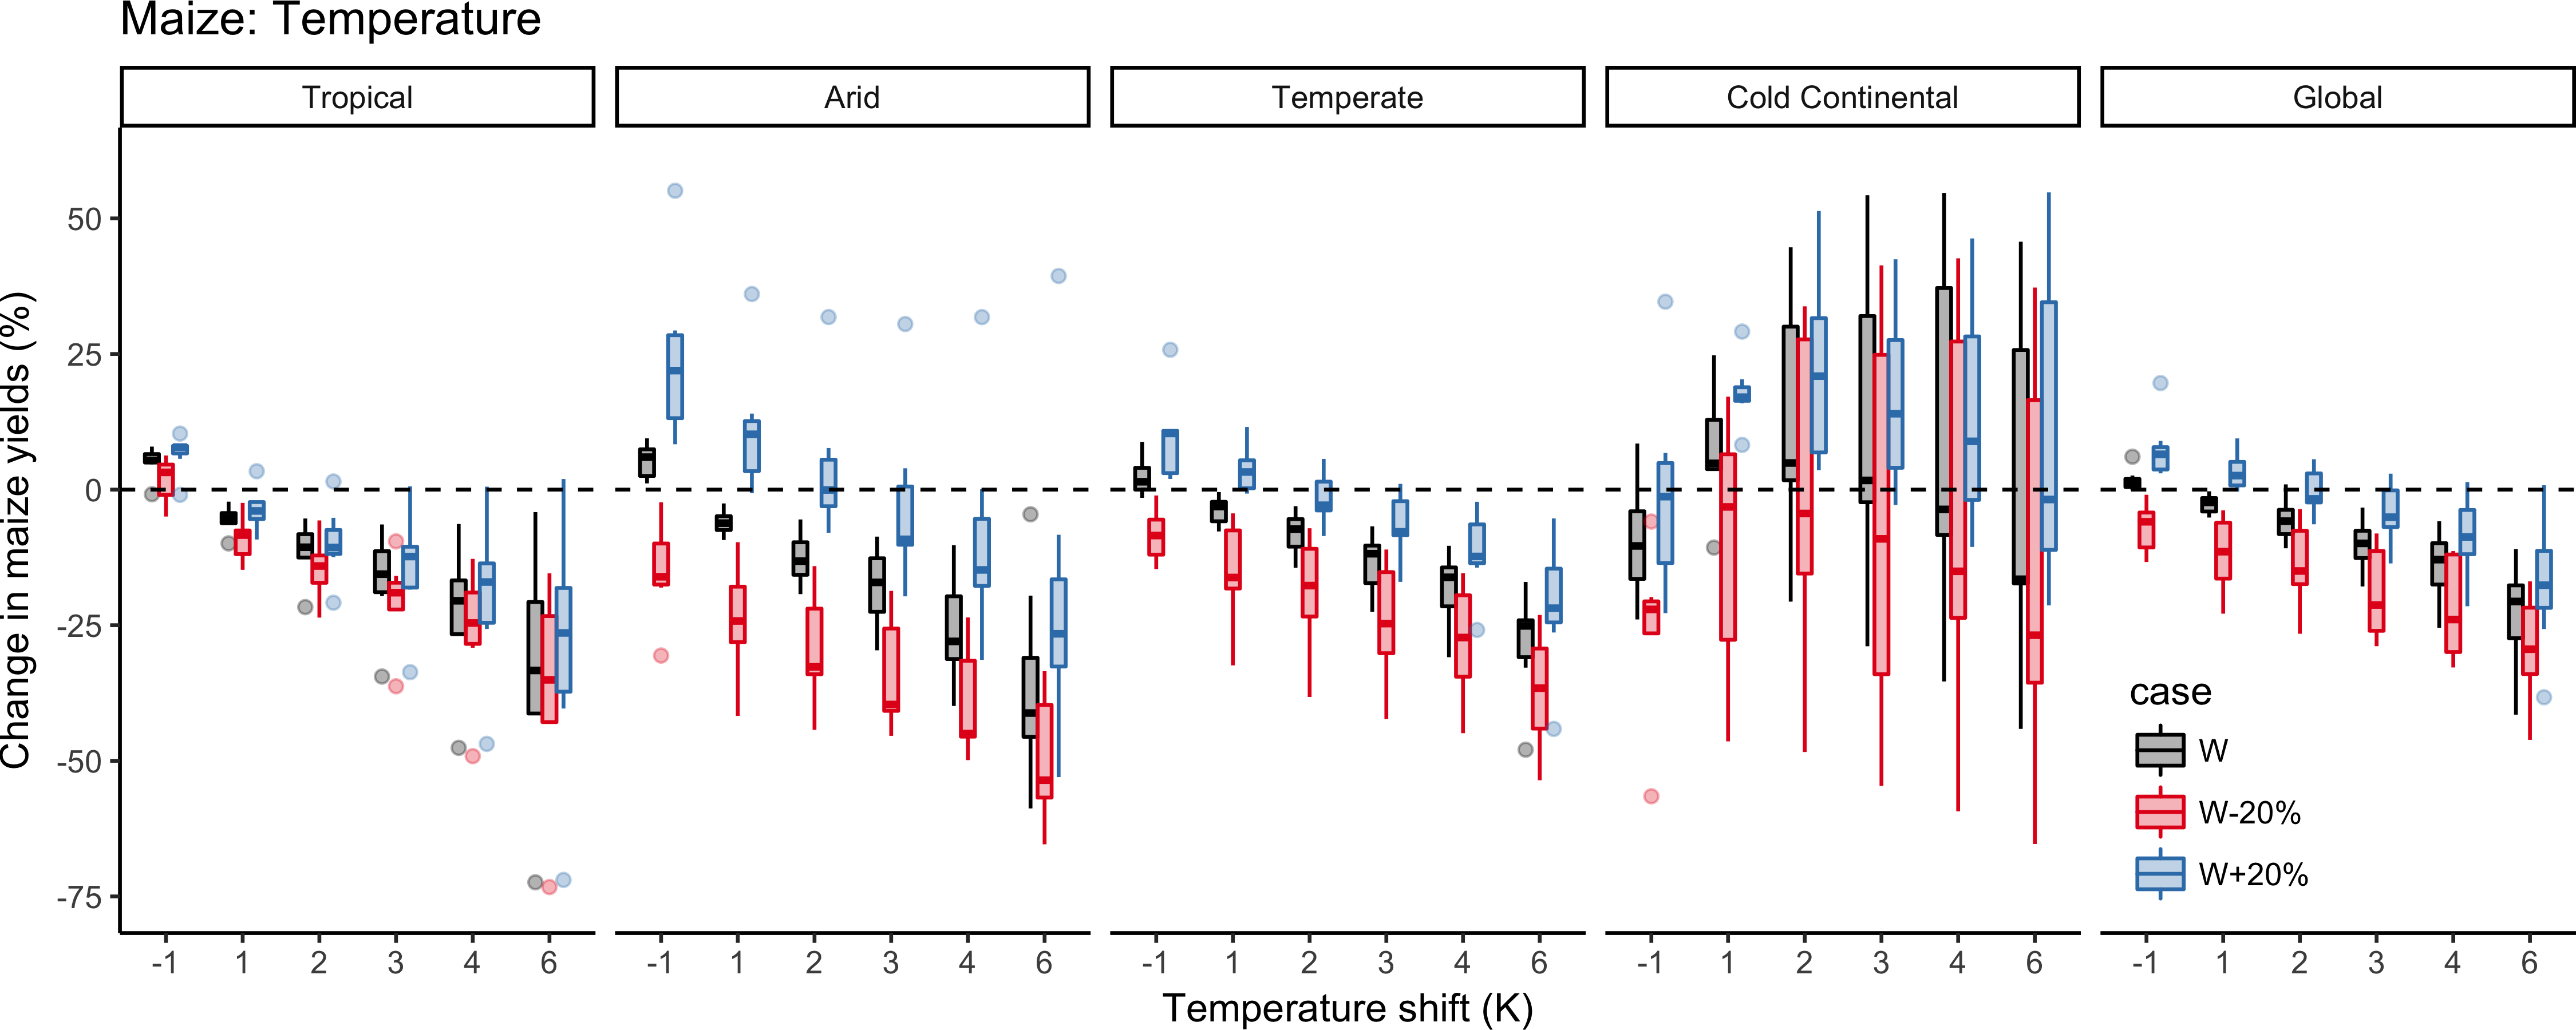
\includegraphics[width=15cm]{figures/maize_sim_CG_T.png}
   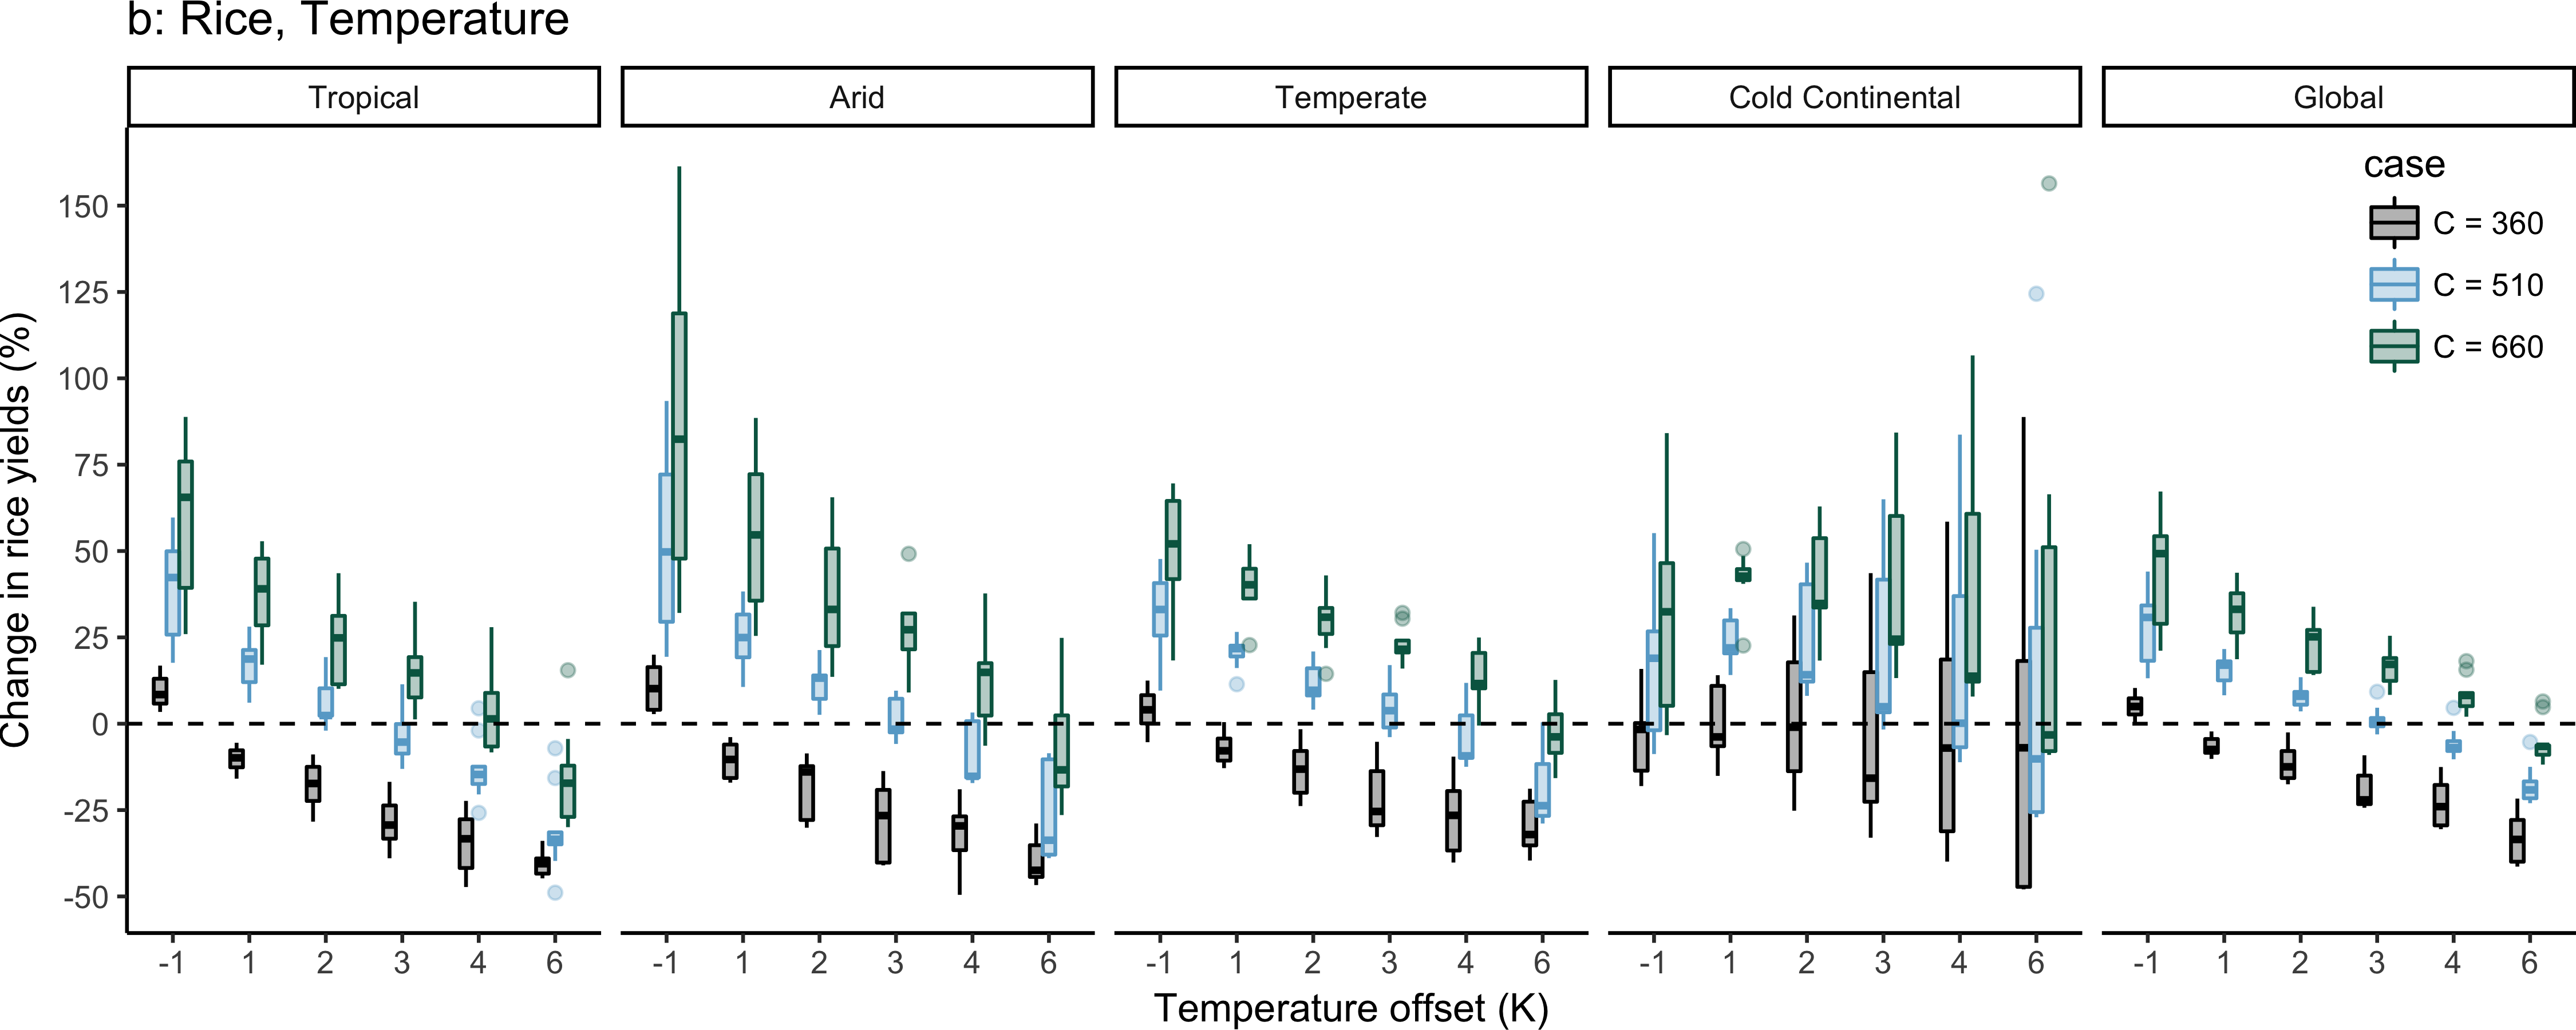
\includegraphics[width=15cm]{figures/rice_sim_CG_T.png}
   \caption{Illustration of the distribution of regional yield changes across the multi-model ensemble, split by K\"{o}ppen-Geiger climate regions \citep{rubel2010}.
  Y-axis is the fractional change in the regional average climatological (30-year mean) potential yield relative to the baseline. Box-and-whiskers plots show distribution across models, with median marked; edges are first and third quartiles; whiskers extend to 1.5$\cdot$IQR.
  Figure shows all modeled land area within each model; see Figure SXX-SXX in the supplemental material for only currently-cultivated land.
  The right panel (Global) shows yield responses to a globally uniform temperature shift; note that these results are not directly comparable to simulations of more realistic climate scenarios.
  Note that \citet{rubel2010} use the name `Snow' rather than `Cold continental'. 
  \textbf{Top:} responses for rainfed maize to applied uniform temperature perturbations, for three discrete precipitation perturbation levels ( -20\%, 0\%, and +20\%), with [CO$_2$] and nitrogen held constant at baseline values (360 pmm and 200 kg ha$^{-1}$ yr$^{-1}$). 
  Outliers in the tropics (strong negative impact of temperature increases) are the pDSSAT model; outliers in the high-rainfall case (strong positive impact of precipitation increases) are the JULES model. 
  Outside high-latitude regions for maize, models generally agree, with projected declines under increasing temperatures larger than inter-model variance. 
  \textbf{Bottom:} Temperature response for irrigated rice for three discrete [CO$_2$] levels, with nitrogen and precipitation held constant. [CO$_2$] does not change the nature of temperature response respective to baseline as the slopes at each [CO$_2$] level are relatively constant.
  There is very little difference across K\"{o}ppen-Geiger regions for irrigated rice.}
   \label{fig:maizerice}
\end{figure*}

\begin{figure*}[ht]
\centering
  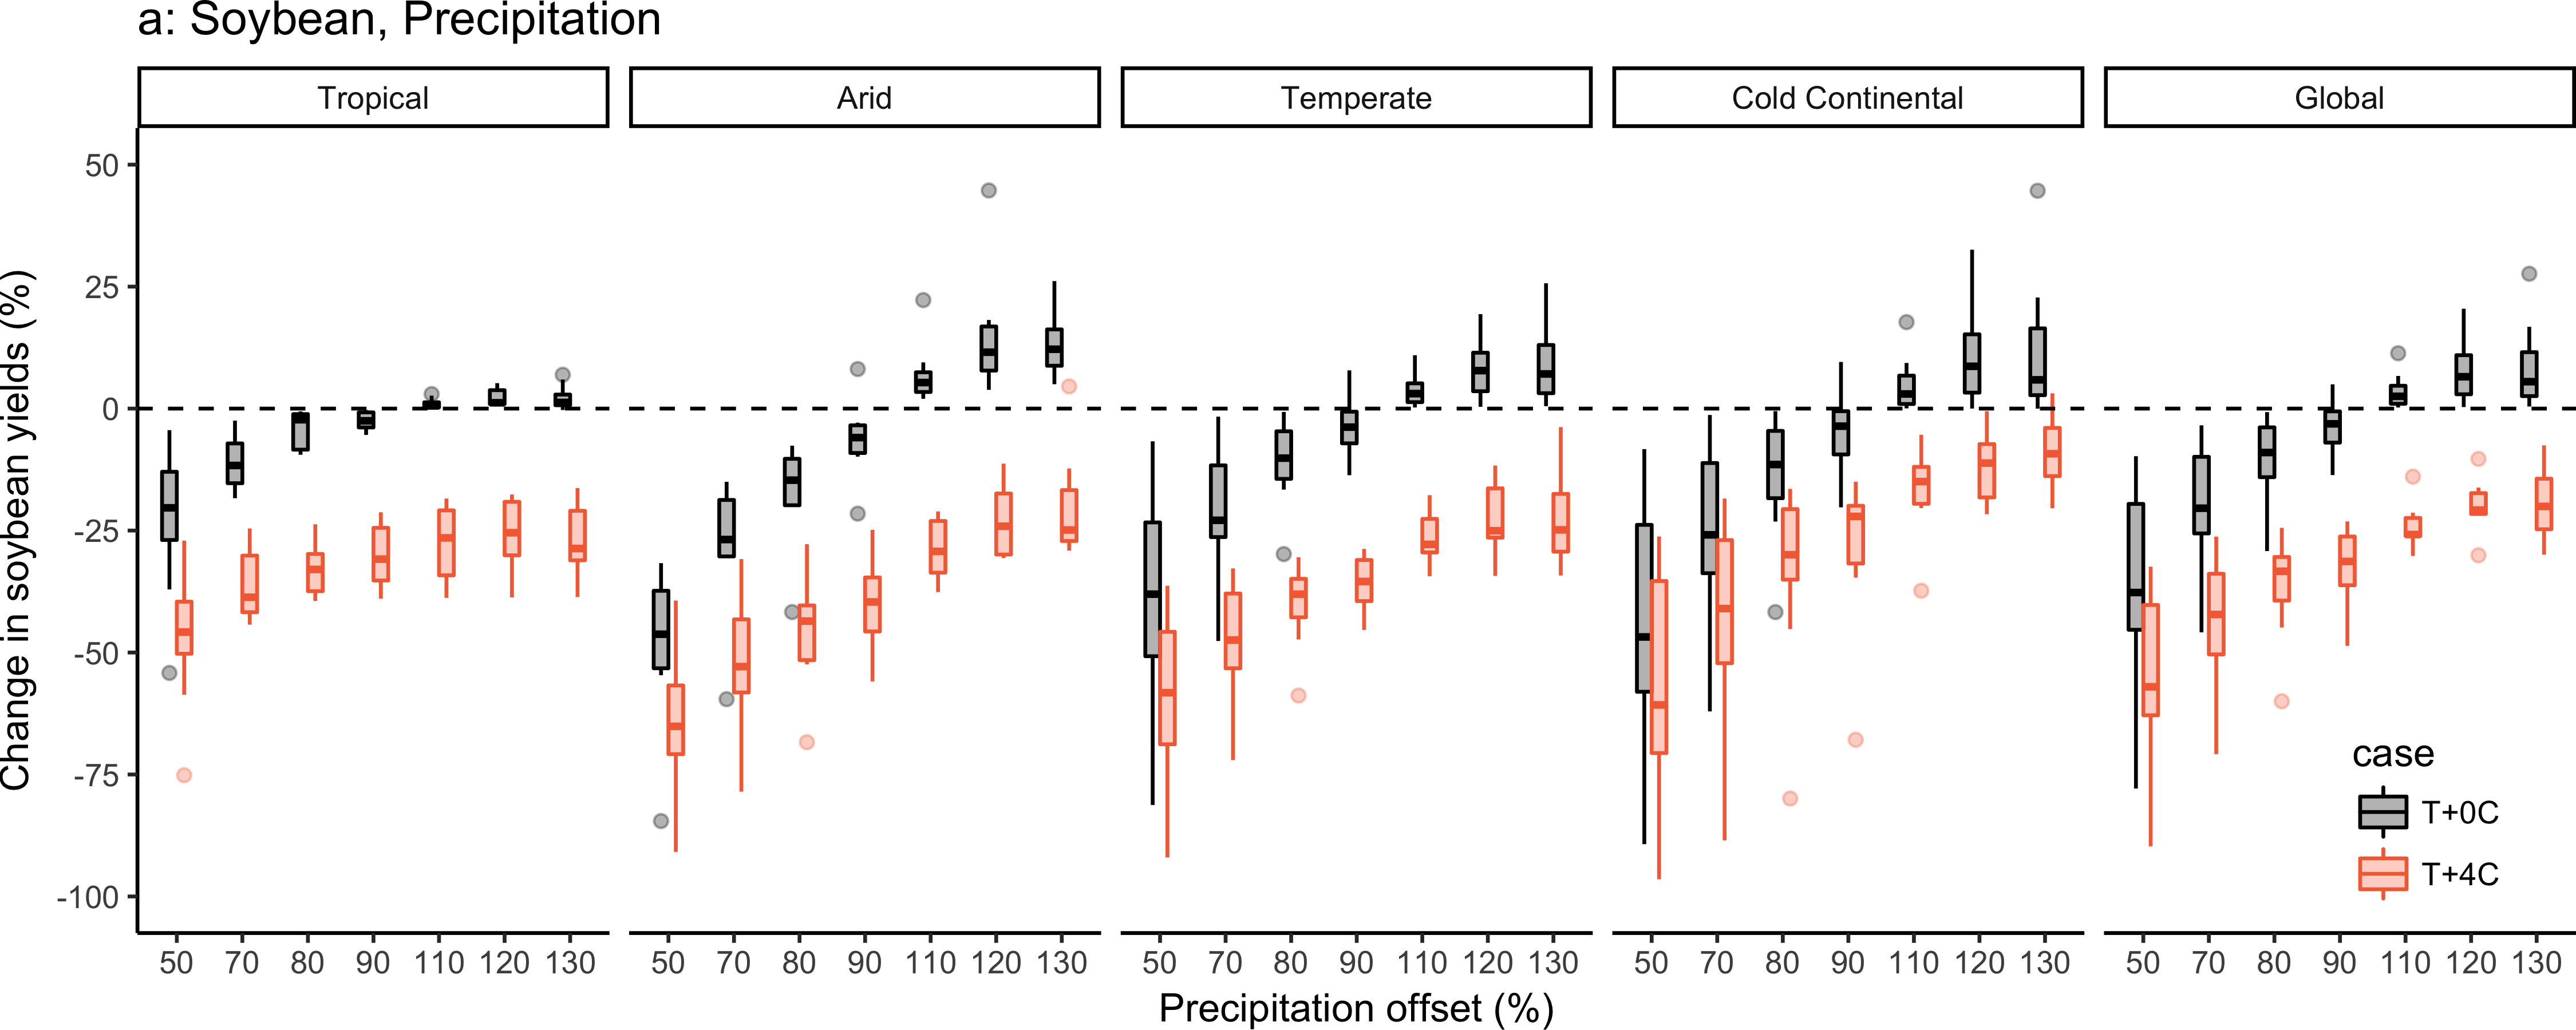
\includegraphics[width=15cm]{figures/soy_sim_CG_W.png}
  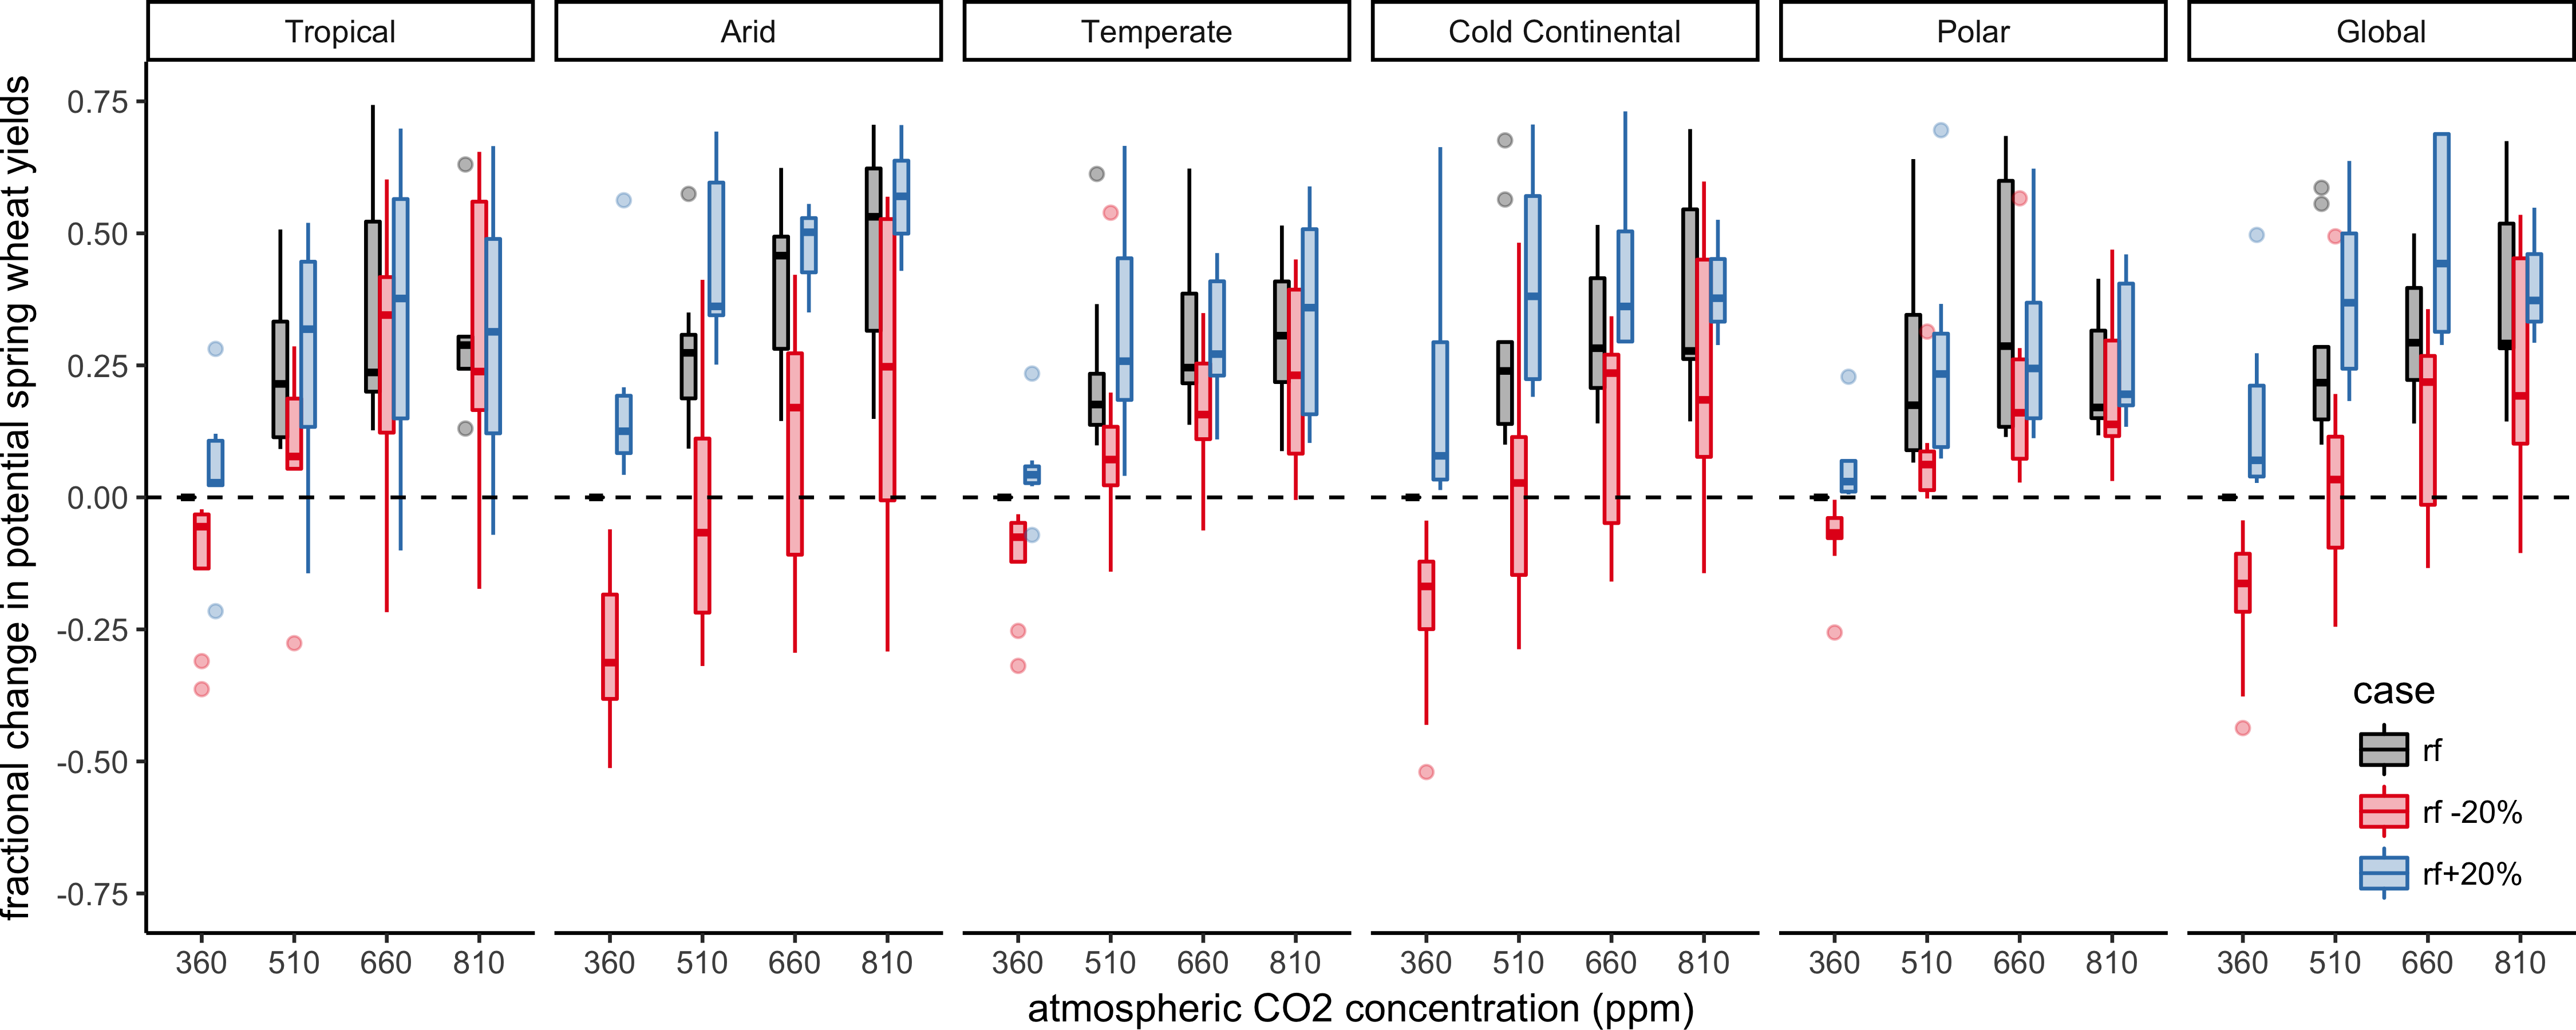
\includegraphics[width=15cm]{figures/swh_sim_CG_C.png}
  \caption{Illustration of the distribution of regional yield changes across the multi-model ensemble, here for soybeans and spring wheat. Conventions as in Figure \ref{fig:maizerice}.
  \textbf{Top:} response for rainfed soy to applied uniform precipitation perturbations, for two discrete temperature levels, with [CO$_2$] and nitrogen held constant at baseline levels. Inter model spread increases for reduced precipitation cases more so than increased precipitation. A leveling out on the increased precipitation side illustrates the saturation effect. Precipitation changes are more important in dryer K\"{o}ppen-Geiger regions, as expected.   Increased temperature tends to flatten the precipitation response in a relative sense because of some prioritizing of the two stresses. 
  \textbf{Bottom:} response for rainfed spring wheat to atmospheric [CO$_2$], for three discrete precipitation perturbation levels with temperature and nitrogen held constant at baseline values.
  The [CO$_2$] 
  Reduced precipitation tends to steepen the [CO$_2$] response and increased precipitation tends to flatten it, as expected. Reduced precipitation tends to increase the inter model spread, especially at the highest [CO$_2$] levels.
   }
   \label{fig:soywheat}
\end{figure*}

Crop models in the GGCMI Phase II ensemble show broadly consistent responses to climate and management perturbations in most regions, with a strong negative impact of increased temperature in all but the coldest regions. 
Mapping the distribution of baseline yields and yield changes shows the geographic dependencies that underlie these results. 
Absolute yield potentials show strong spatial variation, with much of the Earth's surface area unsuitable for any of these crops ((Figure \ref{fig:maizesoybaseline}), left).
Crop yield changes under climate perturbations also show distinct geographic pattern (Figure \ref{fig:maizesoybaseline}, right, which shows fractional yield differences between the T+4 scenario and the baseline scenario with historical climatology).
In general, models agree most on yield response in regions where yield potentials are currently high and therefore where crops are currently grown. 
Models show robust decreases in yields at low latitudes, and highly uncertain median increases at most high latitudes. 

The larger inter-model spread in yield projections at higher latitudes evident in (Figure \ref{fig:maizesoybaseline}) is due in part to how crop suitability or crop failures differ across models. In many cases the spread results from differences in the present-day scenario rather than the future one.  For example, soy yields north of 45$^\circ$ \textcolor{red}{specify if this is on current soybean area only or all areas north of 45$^\circ$?} in the PROMET and LPLmL models are very different in historical simulations -- mostly zero in the PROMET model, which considers present-day temperatures too cold for soy, but averaging 2 tons ha$^{-1}$ in LPJmL -- but become more similar in the T+4 scenario (to mean of \textcolor{red}{XX and XX} tons ha$^{-1}$). Warming increases high-latitude soy yields in PROMET as land becomes suitable for cultivation, but yields in LPJmL actually shift down slightly (Figure \ref{fig:highlat}). Inter-model spreads are largest in wheat projections (Figure SXX), possibly because calibration is most important for wheat \citep[e.g.][]{Asseng2013}.
\textcolor{red}{XXX We need to check if this is due to input climate data difference}
\textcolor{blue}{CM: I don't think we have to. This is a model experiment description paper. The purpose is NOT to expain everything we find in the data.}

We illustrate the across-model spread for selected crops in Figures \ref{fig:maizerice} - \ref{fig:soywheat}, which shows changes in yields across all simulated grid cells for the primary K\"{o}ppen-Geiger climate regions \citep{rubel2010} for various input dimensions.
In warming scenarios with precipitation held constant, all models show decreases in maize yield in the `warm temperate', `equatorial', and `arid' regions that account for nearly three-quarters of global maize production. 
These impacts are robust for even moderate climate perturbations.
In the `warm temperate' zone, even a 1 degree temperature rise with other variables held fixed leads to a median yield reduction that exceeds the variance across models. 
A 6 degree temperature rise results in median loss of $\sim$25\% of yields with a signal to noise ratio of nearly three to one. A notable exception is the `cold continental' region, where models disagree strongly, extending even to the sign of impacts. 
The temperature response is qualitatively similar across all crops included in this study (Figures SX - X).
Increased [CO$_2$] boosts yields overall but does little to change the nature of the temperature response for e.g. irrigated rice (Figure \ref{fig:maizerice}, bottom panel).
Other crops show similar responses to warming, with robust yield losses in warmer locations and high inter-model variance in the `cold continental' regions (Figure SX).

The effects of rainfall changes on yields are also relatively consistent across models (maize: Figure \ref{fig:maizerice}, soybeans: Figure \ref{fig:soywheat}). 
Increased rainfall mitigates the negative effect of higher temperatures by counteracting the increased evapo-transpiration to some degree, most strongly in arid regions.
Decreased rainfall amplifies yield losses and also increases inter-model variance; e.g.\ models agree that the response to decreased water availability is negative in sign but disagree on its magnitude.
Increased temperature results in a relative flattening of the precipitation change response (Figure \ref{fig:soywheat}, top panel).
We show only rainfed maize and soy here; see Figure SXX for comparison between rainfed and irrigated maize. 
As expected, irrigated crops are more resilient to temperature increases in all regions, especially so where water is already limiting. 
The other crops in this study show a qualitatively similar response to changes in precipitation (Figures SX - X).  

Mean climatological yield response to the other two GGCMI Phase II dimensions (C and N) are qualitatively similar across crops. 
The yield response to increased [CO$_2$] for spring wheat is a robust increase across models in all climate regions (Figure \ref{fig:soywheat}, bottom panel). 
Increased precipitation allows crops to capture additional yield boost from elevated [CO$_2$] levels in the mid rage in most climate regions, but this effect saturates at the highest [CO$_2$] levels. 
Increased [CO$_2$] outweighs the damages caused by 20\% reduced precipitation in all climate regions in the multi-model median, but not all models agree upon the positive sign.
Maize has a comparatively muted response to increased [CO$_2$] levels. 

\section{Discussion and Conclusions} 
\label{S:5}
The GGCMI Phase II experiment provides a database designed to allow detailed study of crop yields from process-based models under climate change. 
The use of systematic input parameter variations facilitates not only comparing the sensitivities of process-based crop yield models to changing climate and management inputs but also evaluating the complex interactions between driving factors ([CO$_2$], temperature, precipitation, and applied nitrogen). 
Its global extent also allows identifying geographic shifts in high yield potential locations. 
We expect that the simulations will yield multiple insights in future studies, and show a selection of preliminary results. 
We discuss below the implications from the experimental design, but refrain from analyzing simulation results in detail. 
Data analyses will be conducted in subsequent analyses making use of the GGCMI Phase II data archive.

First, the GGCMI Phase II simulations allow identifying major areas of uncertainty. 
Inter-model uncertainty is qualitatively similar across all four inputs tested at the globally aggregate level with some notable exceptions. 
For example, soybean, a nitrogen-fixing legume, is insensitive to nitrogen addition, while wheat is particularly uncertain in its response to [CO$_2$] levels and water availability (Figure SXX). 
Across geographic regions, projections are most robust in the low latitudes where yield impacts are largest, and most uncertain in the high latitudes where yields may increase under warming. 
Model differences in projected high-latitude yield changes appear driven more by differences in baseline than in responses to CTWN perturbations.  
PROMET, for example, involves a stronger response to cold than does LPJmL, with frost below -8 $^\circ$C irreversibly killing non-winter crops and prolonged periods of below-optimum temperatures also leading to complete crop failure. 
Over the high-latitudes regions simulated by both models, 52\% of grid cells in PROMET report 0 yield in the present climate vs. 11\% of cells in the T+4 scenario, leading to a strong yield gain in warmer future climates. 
In LPJmL outputs, the same high-latitude area is deemed suitable for cultivation even in baseline climate, with crop failure rates of 4\% and 5\% in present and T+4 cases, so that projected yield changes are modest (Figure \ref{fig:highlat}.)

Second, the GGCMI Phase II simulations demonstrate the sensitivity of climate-driven yield impacts to the locations of cultivated land. 
One counterintuitive result apparent in the simulations is that warmer temperatures drive steeper yield reductions in irrigated than rainfed maize when considered only over currently cultivated land, even though water availability increases crop resiliency to temperature increases at any given location (compare Figure \ref{fig:maizerice} and Figures SX to SX). 
The effect results from geographic differences in cultivation: irrigated maize is grown in warmer locations where the impacts of warming are more severe (See Figures SX-SX for other crops.) 
Geographic effects also mean that nitrogen fertilization produces stronger responses in irrigated than non-irrigated wheat and maize, presumably because those rainfed crops are limited by water availability (Figure SX).

Some limitations with the model experiment described here are as follows.
The phase II experiment must not be confused with a correct historic setup, as there is no trend in the [CO$_2$] and the uniform application of 200 kg N ha$^{-1}$ is not representative for many world regions \citep{Elliott2015}.
Some issues with process based models are driven in part by the diversity of new cultivars and genetic variants, which outstrips the ability of academic modeling groups to capture them \citep[e.g.][]{JONES2017b}. 
Models also do not simulate many additional factors affecting production, including but not limited to: pests, diseases, and weeds. 
For these reasons, individual studies must generally re-calibrate models to ensure that short-term predictions reflect current cultivars and management levels. 
The GGCMI Phase II simulations are designed for evaluating changes in yield across the CTNW-A space but not necessarily absolute yields, since they omit detailed calibrations. 

%Inter-model discrepancies are highest in areas not yet cultivated \citep[e.g.][]{Challinor2014, WHITE2011357}, and so projections about shifts in cultivation area under climate change should be made carefully. 

%Finally, process-based models present additional difficulties for high-resolution global studies because of their complexity and computational requirements, as well as the general inability to calibrate site-specific parameters. 
%For global economic impacts assessments, it is often impossible to integrate a set of process-based crop models directly into an integrated assessment model to estimate the potential cost of climate change to the agricultural sector.

In general, the development of multi-model ensembles involving systematic parameters sweeps has large promise for increasing understanding of potential future crop responses and for improving process-based crop models.
The data set is unprecedentedly large, being global in extent, covering 31-simulation years per pixel and up to 756 scenarios for 12 GGCMs.
We expect that the GGCMI Phase II data archive will be used to analyze the different GGCMs' sensitivity to changes in the CTWN-A space, including the interaction between drivers.
The authors are working on some analyses but many more are facilitated by the GGCMI Phase II data archive. 
%We appreciate additional analyses of the data and if the data authors are consulted in the analysis and interpretation of their data. 

%%%%%%%%%%%%%%%%%%%%%%%%%%%%%%%%%%%%%%%%%%%%%%%%%%%%%%%%%%%%%%%
\codedataavailability{The simulation outputs of the mandatory 7 output variables (Table \ref{table:outputs}) are available on zenodo.org. 
See Appendix \ref{A:1} for data DOIs. 
All other simulation output variables are available upon request to the corresponding author. 
The scripts for generating the spring wheat and winter wheat growing seasons and second fertilizer dates and the quality screening script is available at https://github.com/RDCEP/ggcmi/blob/phase2/.
All input data are available via globus.org (registration required, free of charge):
Minimum cropland mask is available at
\url{https://app.globus.org/file-manager?origin_id=e4c16e81-6d04-11e5-ba46-22000b92c6ec&origin_path=\%2FAgMIP.input\%2Fother.inputs\%2Fphase2.masks\%2F}
choose the file boolean\_cropmask\_ggcmi\_phase2.nc4
Growing period data for wheat is now divided up into winter and spring wheat, available at
\url{https://app.globus.org/file-manager?origin_id=e4c16e81-6d04-11e5-ba46-22000b92c6ec&origin_path=\%2FAgMIP.input\%2Fother.inputs\%2FAGMIP_GROWING_SEASON.HARM.version2.0\%2F}
whereas all other growing season data (maize, rice, soybean) are the same as in Phase I (version 1.25), available at
\url{https://app.globus.org/file-manager?origin_id=e4c16e81-6d04-11e5-ba46-22000b92c6ec&origin_path=\%2FAgMIP.input\%2Fother.inputs\%2FAGMIP_GROWING_SEASON.HARM.version1.25\%2F}
}

\appendix
\section{}
\subsection{Data Access}
\label{A:1}
Simulation yield output datasets can be found at the DOIs located in table \ref{table:dataloc}. 
Data are published in crop- and GGCM-specific packages, in order to break down the overall data amount into manageable packages (<50GB per archive).

\begin{table*}[t]
\caption{DOI's for model yield data outputs. All yield output data can be found at https://doi.org/10.5281/zenodo/XX. Where XX is the value found in the table.} 
\label{table:dataloc}
  \begin{tabular}{p{3cm} p{1.5cm} p{1.5cm} p{1.5cm} p{1.5cm} p{1.5cm}}
        \tophline
        {\textbf{Model}}&{\textbf{Maize}}&{\textbf{Soybean}}&{\textbf{Rice}}&{\textbf{Winter wheat}}&{\textbf{Spring wheat}}\\ \middlehline
        {\textbf{APSIM-UGOE}} & {2582531} & {2582535} & {2582533} & {2582537} & {2582539}\\ \middlehline
        {\textbf{CARAIB}} & {2582522} & {2582508} & {2582504} & {2582516} & {2582499}\\ \middlehline
        {\textbf{EPIC-IIASA}} & {2582453} & {2582461} & {2582457} & {2582463} & {2582465}\\  \middlehline
        {\textbf{EPIC-TAMU}} & {2582349} & {2582367} & {2582352} & {2582392} & {2582418}\\ \middlehline
        {\textbf{JULES}} & {2582543} & {2582547} & {2582545} & {--} & {2582551}\\ \middlehline
        {\textbf{GEPIC}} & {2582247} & {2582258} & {2582251} & {2582260} & {2582263}\\ \middlehline
        {\textbf{LPJ-GUESS}} & {2581625} & {--} & {--} & {2581638} & {2581640}\\  \middlehline
        {\textbf{LPJmL}} & {2581356} & {2581498} & {2581436} & {2581565} & {2581606}\\ \middlehline
        {\textbf{ORCHIDEE-crop}} & {2582441} & {--} & {2582445} & {2582449} & {--}\\ \middlehline
        {\textbf{pDSSAT}} & {2582111} & {2582147} & {2582127} & {2582163} & {2582178}\\ \middlehline
        {\textbf{PEPIC}} & {2582341} & {2582433} & {2582343} & {2582439} & {2582455}\\ \middlehline
        {\textbf{PROMET}} & {2582467} & {2582488} & {2582479} & {2582490} & {2582492}\\
        \bottomhline
    \end{tabular}
\end{table*}
\noappendix %% use this to mark the end of the appendix section

\authorcontribution{J.E., C.M, and A.R.\ designed the research. C.M., J.J., J.B., P.C., M.D., P.F., C.F., L.F., M.H., C.I., I.J., C.J., N.K., M.K., W.L., S.O., M.P., T.P., A.R., X.W., K.W., and F.Z.\ performed the simulations. J.F., J.J., A.S., M.L., C.M., and E.M.\ performed the analysis and J.F., E.M., and C.M.\ prepared the manuscript.}

\competinginterests{The authors declare no competing interests.}

\begin{acknowledgements}
This research was performed as part of the Center for Robust Decision-Making on Climate and Energy Policy (RDCEP) at the University of Chicago, and was supported through a variety of sources. 
RDCEP is funded by NSF grant \#SES-1463644 through the Decision Making Under Uncertainty program. 
J.F.\ was supported by the NSF NRT program, grant \#DGE-1735359. 
C.M.\ was supported by the MACMIT project (01LN1317A) funded through the German Federal Ministry of Education and Research (BMBF). 
C.F.\ was supported by the European Research Council Synergy grant \#ERC-2013-SynG-610028 Imbalance-P. 
P.F.\ and K.W.\ were supported  by the Newton Fund through the Met Office Climate Science for Service Partnership Brazil (CSSP Brazil). 
K.W.\ was supported by the IMPREX research project supported by the European Commission under the Horizon 2020 Framework programme, grant \#641811. 
A.S.\ was supported by the Office of Science of the U.S. Department of Energy as part of the Multi-sector Dynamics Research Program Area. 
S.O.\ acknowledges support from the Swedish strong research areas BECC and MERGE together with support from LUCCI (Lund University Centre for studies of Carbon Cycle and Climate Interactions). 
R.C.I.\ acknowledges support from the Texas Agrilife Research and 634 Extension, Texas A \&M University. This is paper number 35 of the Birmingham Institute of Forest Research. Computing resources were provided by the University of Chicago Research Computing Center (RCC).
\end{acknowledgements}

%% Since the Copernicus LaTeX package includes the BibTeX style file copernicus.bst,
\bibliographystyle{copernicus}
\bibliography{bib}

\end{document}
%%%%%%%%%%%%%%%%%%%%%%%%%%%%%%%%%%%%%%%%%%%%%%%%%%%%%%%%%%%%%%%%%%%%%%%%%%%%%%%%%%
%%%%%%%%%%%%%%%%%%%%%%%%%%%%%%%%%%%%%%%%%%%%%%%%%%%%%%%%%%%%%%%%%%%%%%%%%%%%%%%%%%
%%%%%%%%%%%%%%%%%%%%%%%%%%%%%%%%%%%%%%%%%%%%%%%%%%%%%%%%%%%%%%%%%%%%%%%%%%%%%%%%%%
%%%%%%%%%%%%%%%%%%%%%%%%%%%%%%%%%%%%%%%%%%%%%%%%%%%%%%%%%%%%%%%%%%%%%%%%%%%%%%%%%%

%%%%%%%%%%%%%%%%%%%%%%%%%%%%%%%%%%%%%%%%%%%%%%%%%%%%%%%%%%%%%%%%%%%%%%%%%%%%%%%%%%
%%%%%%%%%%%%%%%%%%%%%%%%%%%%%%%%%%%%%%%%%%%%%%%%%%%%%%%%%%%%%%%%%%%%%%%%%%%%%%%%%%
%%%%%%%%%%%%%%%%%%%%%%%%%%%%%%%%%%%%%%%%%%%%%%%%%%%%%%%%%%%%%%%%%%%%%%%%%%%%%%%%%%
%%%%%%%%%%%%%%%%%%%%%%%%%%%%%%%%%%%%%%%%%%%%%%%%%%%%%%%%%%%%%%%%%%%%%%%%%%%%%%%%%%
%%%%%%%%%%%%%%%%%%%%%%%%%%%%%%%%%%%%%%%%%%%%%%%%%%%%%%%%%%%%%%%%%%%%%%%%%%%%%%%%%%
%%%%%%%%%%%%%%%%%%%%%%%%%%%%%%%%%%%%%%%%%%%%%%%%%%%%%%%%%%%%%%%%%%%%%%%%%%%%%%%%%%
%%%%%%%%%%%%%%%%%%%%%%%%%%%%%%%%%%%%%%%%%%%%%%%%%%%%%%%%%%%%%%%%%%%%%%%%%%%%%%%%%%
%%%%%%%%%%%%%%%%%%%%%%%%%%%%%%%%%%%%%%%%%%%%%%%%%%%%%%%%%%%%%%%%%%%%%%%%%%%%%%%%%%
%%%%%%%%%%%%%%%%%%%%%%%%%%%%%%%%%%%%%%%%%%%%%%%%%%%%%%%%%%%%%%%%%%%%%%%%%%%%%%%%%%
%%%%%%%%%%%%%%%%%%%%%%%%%%%%%%%%%%%%%%%%%%%%%%%%%%%%%%%%%%%%%%%%%%%%%%%%%%%%%%%%%%
%%%%%%%%%%%%%%%%%%%%%%%%%%%%%%%%%%%%%%%%%%%%%%%%%%%%%%%%%%%%%%%%%%%%%%%%%%%%%%%%%%
%%%%%%%%%%%%%%%%%%%%%%%%%%%%%%%%%%%%%%%%%%%%%%%%%%%%%%%%%%%%%%%%%%%%%%%%%%%%%%%%%%
%%%%%%%%%%%%%%%%%%%%%%%%%%%%%%%%%%%%%%%%%%%%%%%%%%%%%%%%%%%%%%%%%%%%%%%%%%%%%%%%%%
%%%%%%%%%%%%%%%%%%%%%%%%%%%%%%%%%%%%%%%%%%%%%%%%%%%%%%%%%%%%%%%%%%%%%%%%%%%%%%%%%%
%%%%%%%%%%%%%%%%%%%%%%%%%%%%%%%%%%%%%%%%%%%%%%%%%%%%%%%%%%%%%%%%%%%%%%%%%%%%%%%%%%
%%%%%%%%%%%%%%%%%%%%%%%%%%%%%%%%%%%%%%%%%%%%%%%%%%%%%%%%%%%%%%%%%%%%%%%%%%%%%%%%%%


The 12 models included in GGCMI Phase II are all process-based crop models that are widely used in impacts assessments (Table \ref{table:models}). 
Although some models share a common base (e.g.\ the LPJ family or the EPIC family of models), they have subsequently developed independently. 
Differences in model structure mean that several key factors are not standardized across the experiment, such as carry-over effects across growing years including residue management and soil moisture, and the extent of simulated area for different crops. 
Not all modeling teams provide the full simulation protocol, for instance, CARIAB and JULES do not simulate the nitrogen dimension and some crops are not parameterized in each model (see Table \ref{table:models} for details). 
%Note that the three models that provide less than 50 simulations are excluded from the emulator analysis (APSIM-UGOE, EPIC-IIASA, and ORCHIDEE-crop).
%The different levels in carbon dioxide (n=4), temperature (n=7), water availability (n=9), and nitrogen application (n=3) combine to a total of 756 CTWN combinations.
%For these CTWN combinations models conducted global gridded simulations of 31 years per crop, but not all crop models were able to provide the full set. 
%One important aspect of climate change impacts on crop yields is the acceleration of crop phenology under warming that can be addressed with slower maturing varieties. 
%The GGCMI Phase II experiment thus also includes an additional adaptation set with 648 CTWN elements assuming new varieties which regain the original growing season in each location. 


%\begin{comment}
% ---- SAVE FOR DISCUSSION
%These issues are driven in part by the diversity of new cultivars and genetic variants, which outstrips the ability of academic modeling groups to capture them \citep[e.g.][]{JONES2017b}. 
%Models also do not simulate many additional factors affecting production, including but not limited to: pests, diseases, and weeds. 
%For these reasons, individual studies must generally re-calibrate models to ensure that short-term predictions reflect current cultivars and management levels. 
Inter-model discrepancies can also be high in areas not yet cultivated \citep[e.g.][]{Challinor2014, WHITE2011357}. 
Finally, process-based models present additional difficulties for high-resolution global studies because of their complexity and computational requirements, as well as the general inability to calibrate site-specific parameters. 
%For global economic impacts assessments, it is often impossible to integrate a set of process-based crop models directly into an integrated assessment model to estimate the potential cost of climate change to the agricultural sector.

This must not be confused with a correct historic setup, as there is no trend in the [CO$_2$] and the uniform application of 200 kg N ha$^{-1}$ is not representative for many world regions \citep{Elliott2015}.
The GGCMI Phase II simulations are designed for evaluating changes in yield across the CTNW-A space but not necessarily absolute yields, since they omit detailed calibrations. 
To provide some evaluation of the skill of the process-based models used, we repeat the evaluation exercises of \citet{muller_global_2017} for GGCMI Phase I but stress that in particular the uniform fertilizer application does not represent the actual situation.

\end{comment}

% to me, this is too broad of an introduction and the distinction of different modle types is more suitable for pitching the emulators than for the introduction of the experiment

%Computational models have been used to project crop yields since the 1950's, beginning with statistical models  that attempt to capture the relationship between input factors and resultant yields \citep[e.g.][]{Heady57, Heady61}. 
%These statistical models were typically developed on a small scale for locations with extensive histories of yield data. 
%The emergence of electronic computers allowed development of numerical models that simulate the process of photosynthesis and the biology and phenology of individual crops (first proposed by \citet{wit58} and \citet{Duncan67} and attempted by \citet{Duncan72}; for a history of crop model development see \citet{Rosenzweig2014}). 
%A half-century of improvement in both models and computing resources means that researchers can now run crop simulations for many years at higher spatial resolution on the global scale. 


%The Global Gridded Crop Model Intercomparison (GGCMI) Phase II experiment was conducted by a suite of process-based crop models, running across historical conditions perturbed by a set of discrete steps in the four input parameters (CTWN), for both adaptation settings (yes/no). 
%The experimental protocol involves 756 different parameter combinations for each model and crop for the non-adapted and 648 combinations for the adapted setting (does not include T=0), with simulations providing near-global coverage at a half degree spatial resolution. 
%The experiment was conducted as part of the Agricultural Model Intercomparison and Improvement Project (AgMIP) \citep{ROSENZWEIG2013, Rosenzweig2014}, an international effort conducted under a framework similar to the Climate Model Intercomparison Project (CMIP) \citep{Taylor2012, Eyring2016}. 
%The GGCMI protocol builds on the AgMIP Coordinated Climate-Crop Modeling Project (C3MP) \citep{ruane2014, mcdermid2015agmip} and contributes to the AgMIP Coordinated Global and Regional Assessments (CGRA) \citep{ruane2018, rosenzweig2018}. 
%GGCMI Phase II is designed to allow addressing goals such as understanding where highest-yield regions may shift under climate change; exploring future adaptive management strategies; understanding how interacting input drivers affect crop yield; quantifying uncertainties across models and major drivers; and testing strategies for producing lightweight emulators of process-based models. 

\begin{figure*}[ht]
\centering
   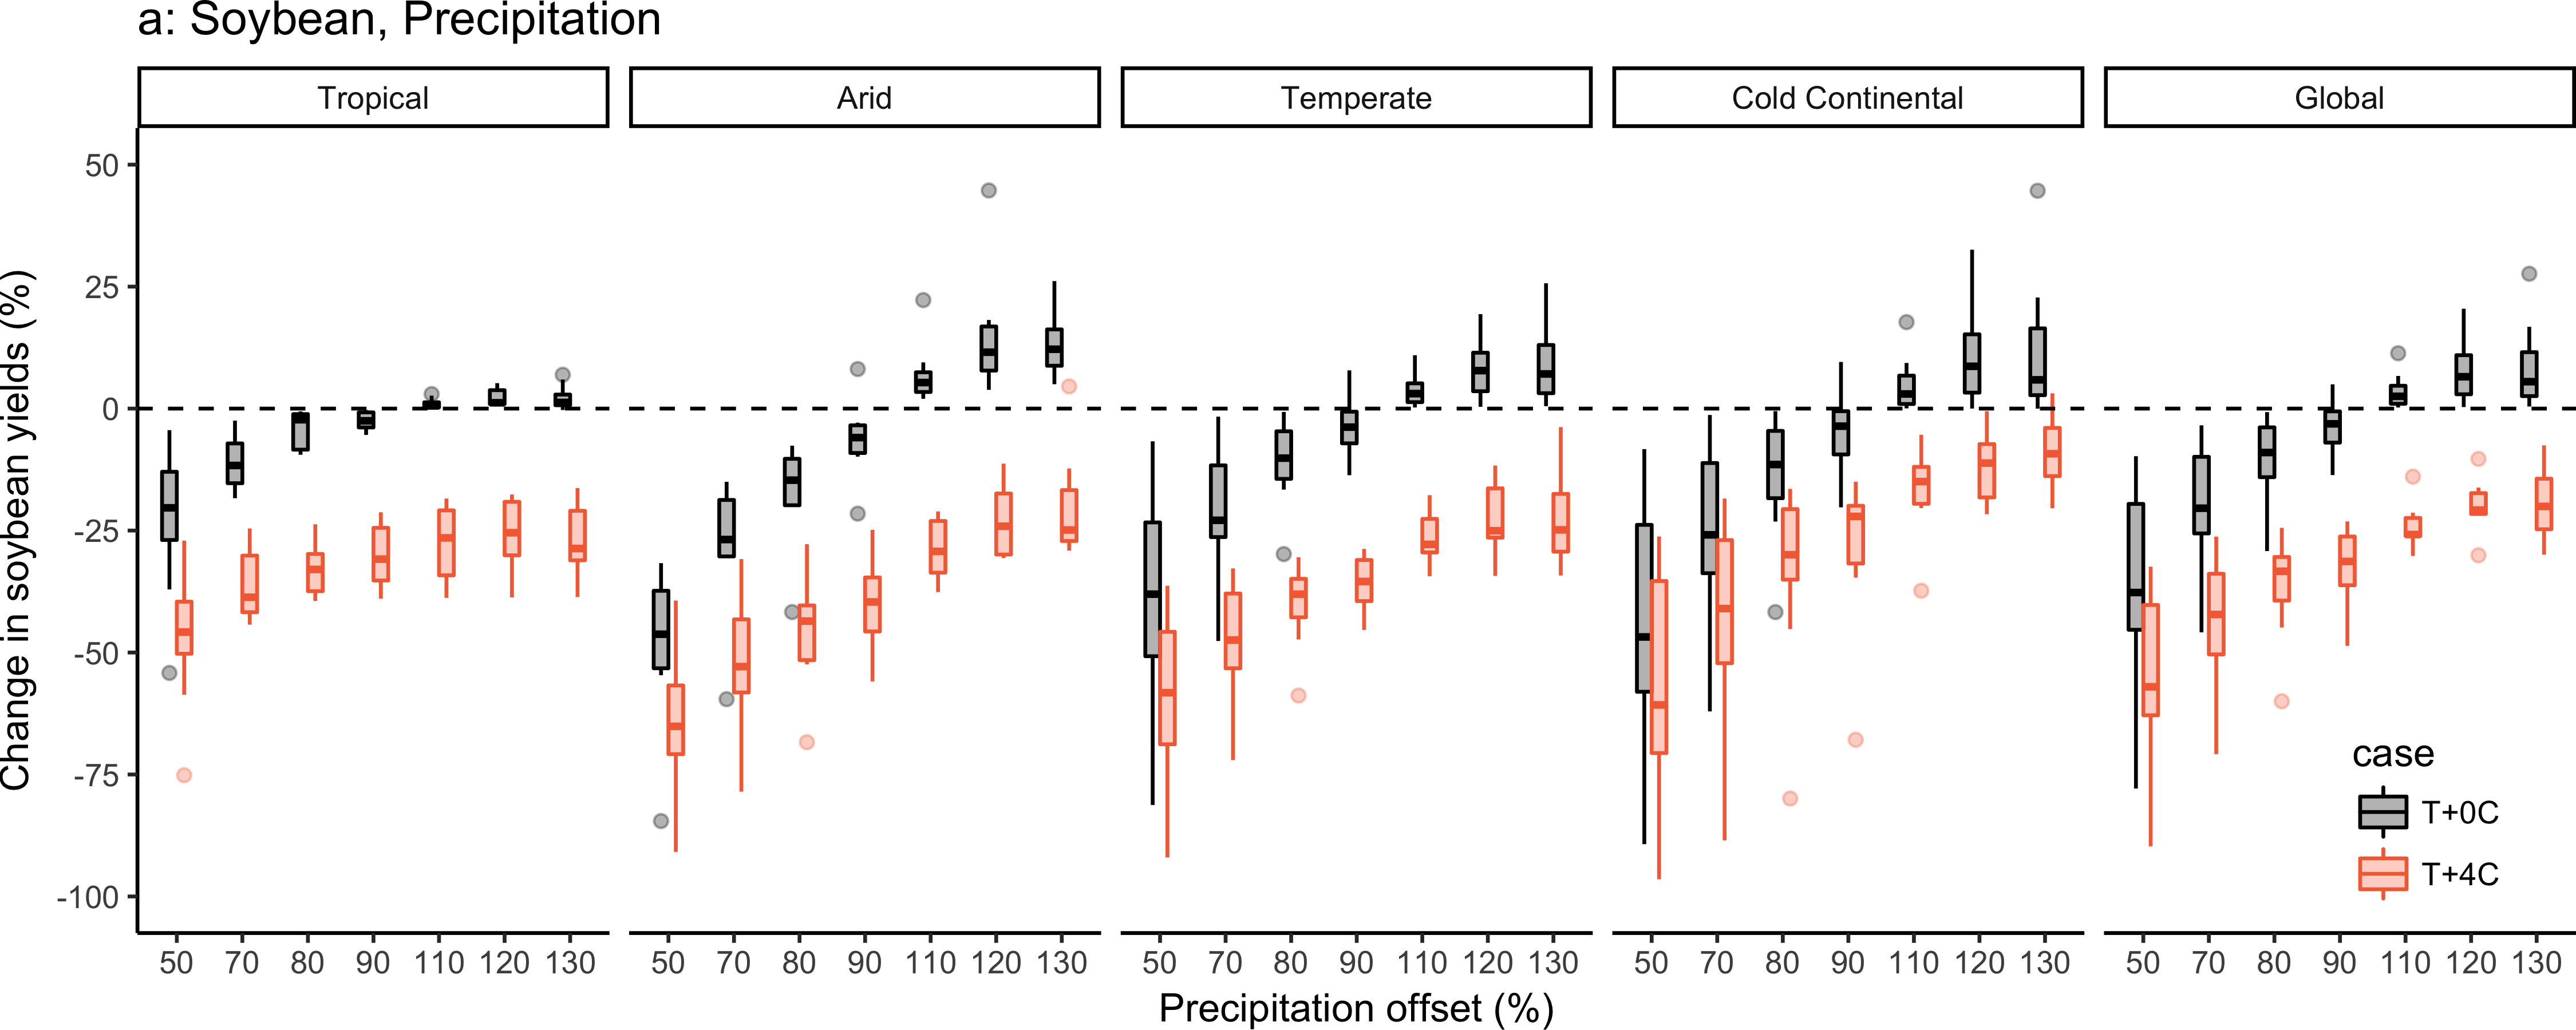
\includegraphics[width=15cm]{figures/soy_sim_CG_W.png}
   \caption{Illustration of the distribution of regional yield changes across the multi-model ensemble, split by K\"{o}ppen-Geiger climate regions for soybean. Same conventions as Figure \ref{fig:globesim} except precipitation is varied. Simulations at a T + 4K are show in color.}
   \label{fig:globesim_W}
\end{figure*}

\begin{figure*}[ht]
\centering
   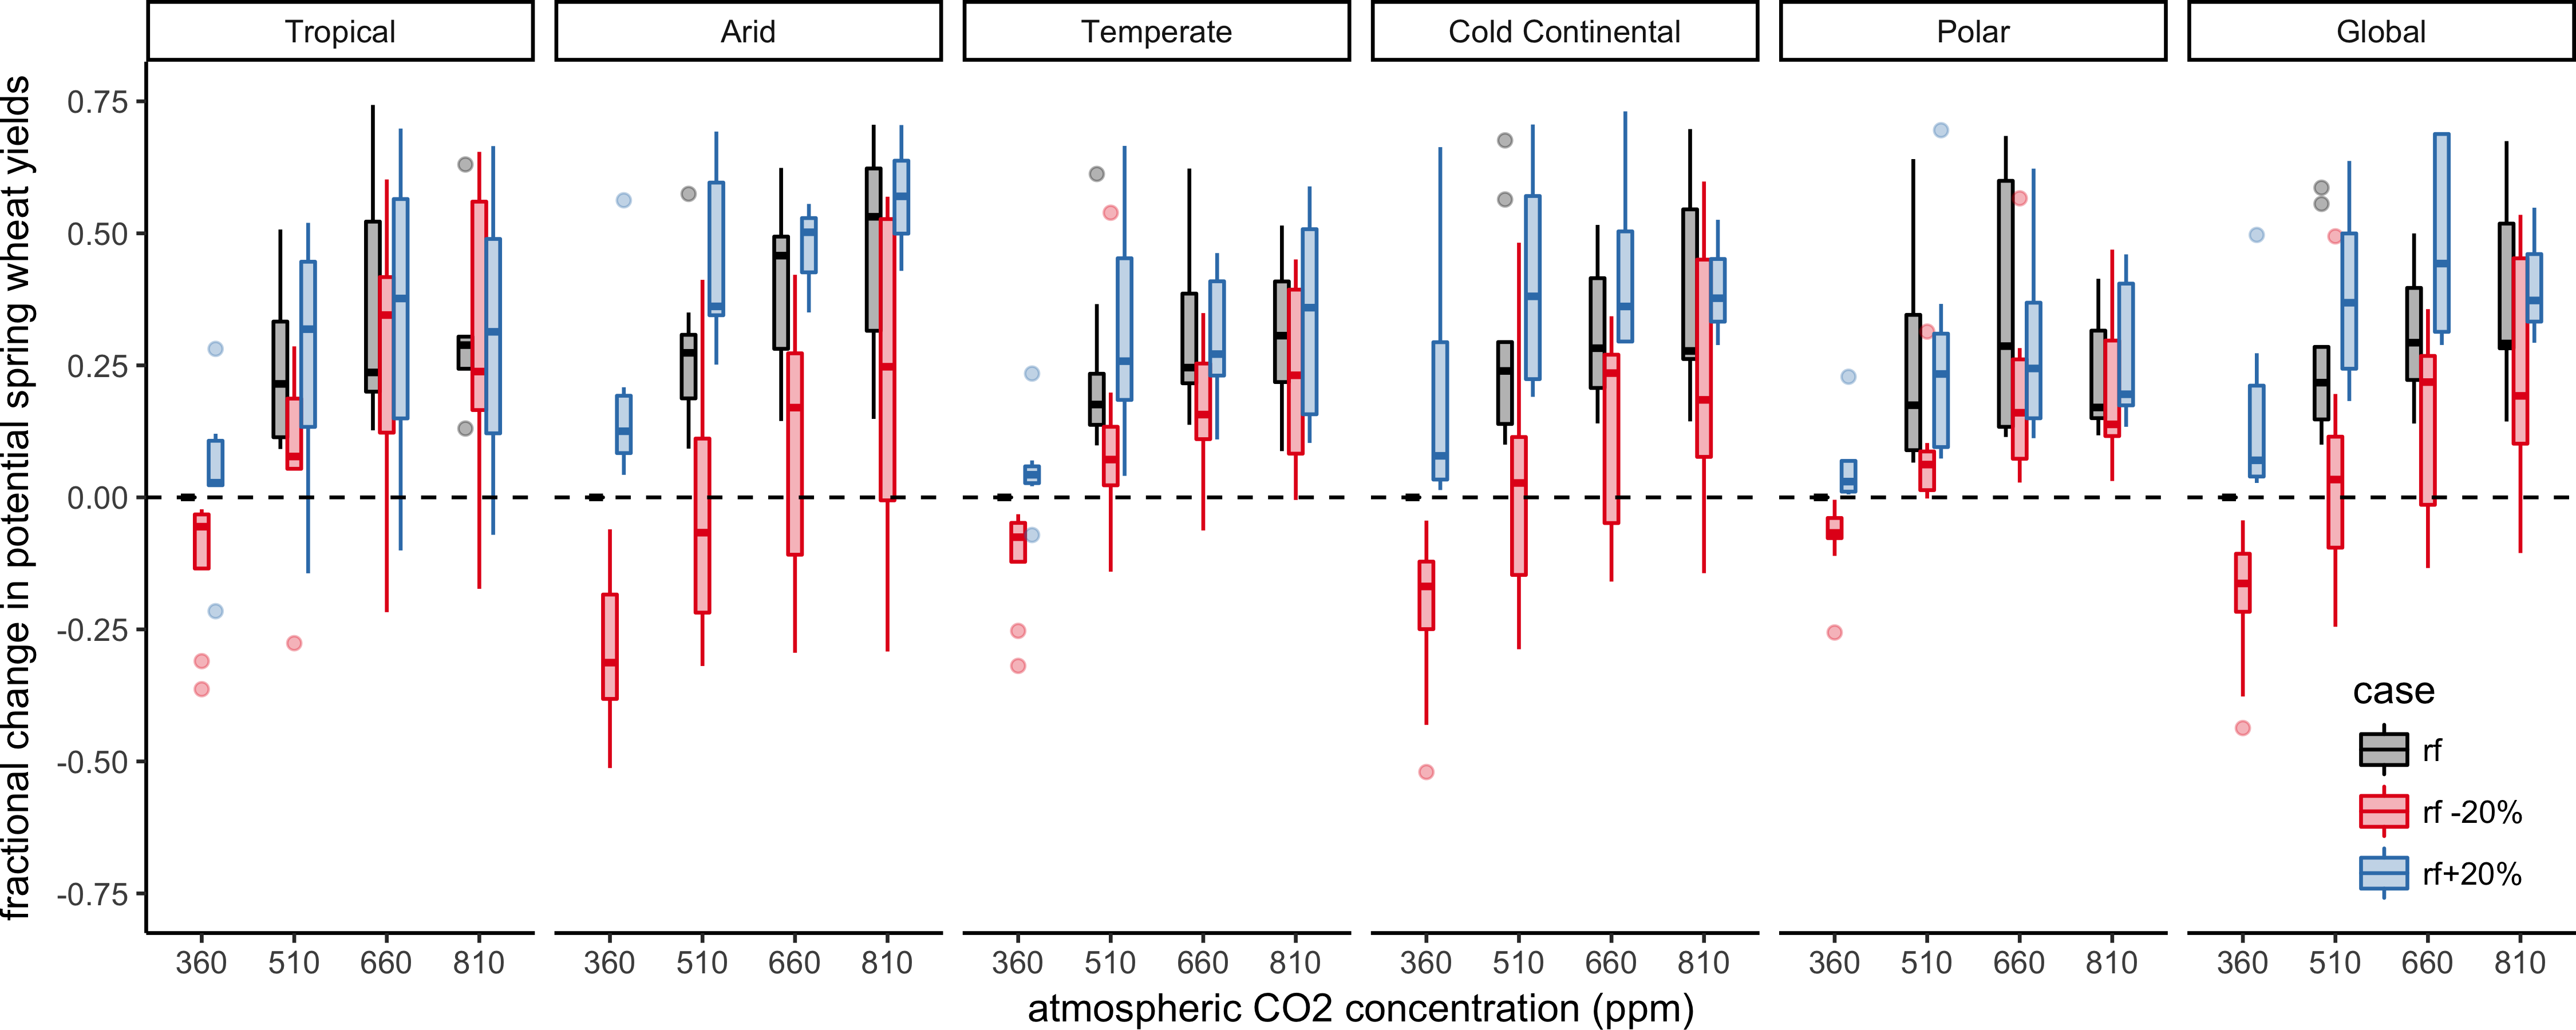
\includegraphics[width=15cm]{figures/swh_sim_CG_C.png}
   \caption{Illustration of the distribution of regional yield changes across the multi-model ensemble, split by K\"{o}ppen-Geiger climate regions for spring wheat. Same conventions as Figure \ref{fig:globesim} except atmospheric carbon dioxide is varied. Two different water specifications (historical precipitation -20\% and +20\%) are shown in colors.}
   \label{fig:globesim_C}
\end{figure*}

\begin{figure*}[ht]
\centering
   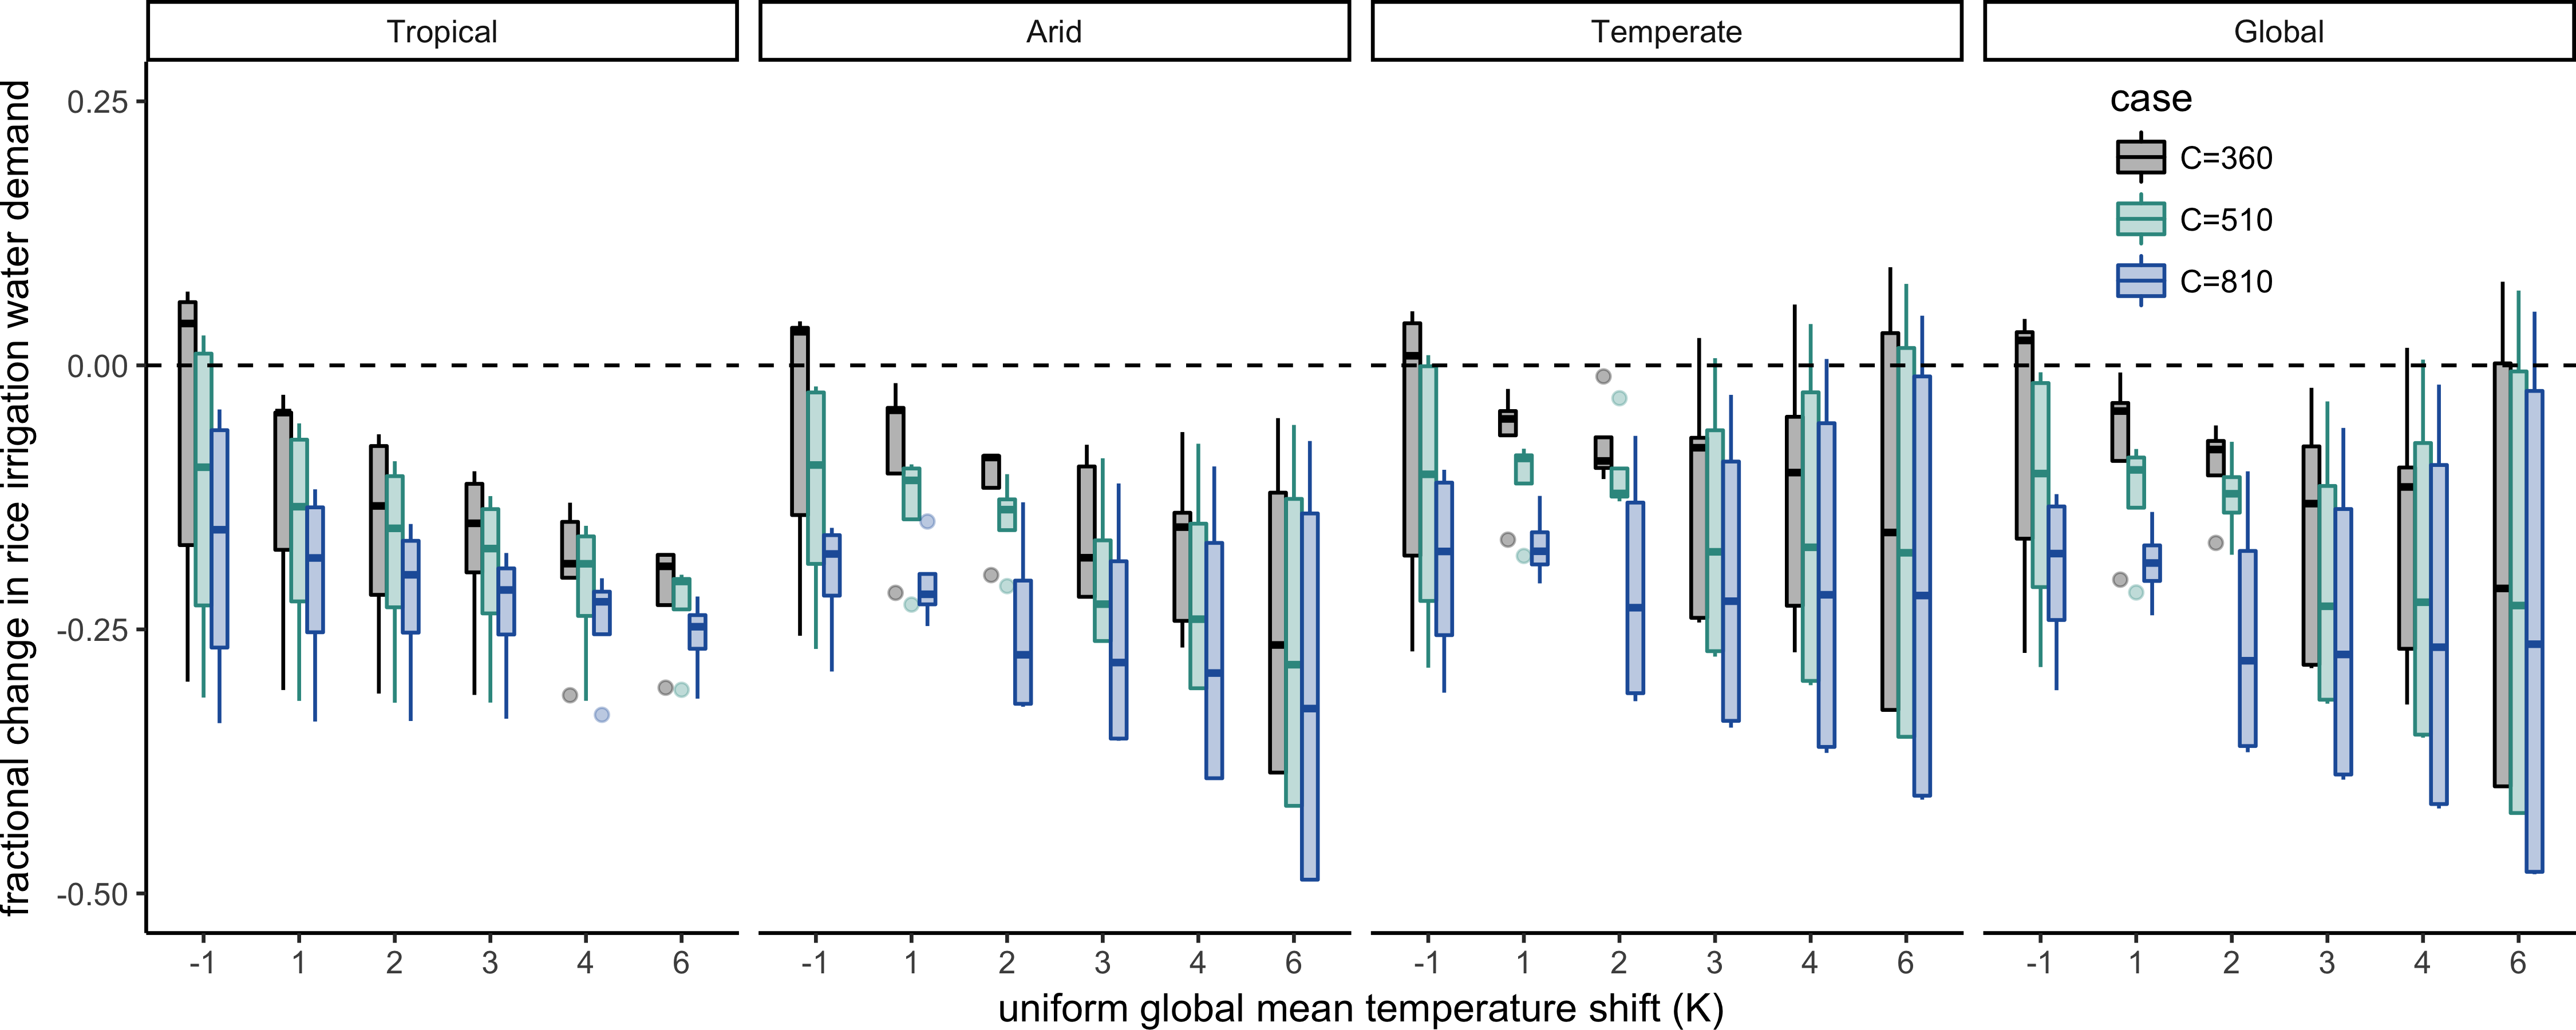
\includegraphics[width=14cm]{figures/rice_sim_CG_irrwat.png}
   \caption{Illustration of the distribution of regional irrigation water demand across the multi-model ensemble, split by K\"{o}ppen-Geiger climate regions for rice. Cold continental and polar regions are not shown because very little rice is grown in these regions.}
   \label{fig:globesim_IRR}
\end{figure*}

Simulated irrigation water demand, as an example for non-yield outputs, is also variable across models and shows mixed responses to increasing temperatures and generally a decrease with increasing levels of [CO$_2$] (Figure \ref{fig:globesim_IRR}). 
This is because shorter growing seasons under warming reduce water demand whereas warmer temperatures increase water demand. 
Often, the inter-model uncertainty is larger than the response to warming and can both increase (e.g. Arid) or decrease (e.g. Tropical) with warming.
